
\documentclass[10pt,a4paper]{article}

\usepackage[T1]{fontenc}
\usepackage[utf8]{inputenc}
\usepackage{lmodern}
\usepackage[english]{babel}
\usepackage{microtype}

\DisableLigatures[-]{family = tt*}

\usepackage[a4paper,top=2.1cm,bottom=2.1cm,left=2cm,right=2cm,headheight=14pt]{geometry}
\usepackage{fancyhdr}
\setlength{\parskip}{0.35em}
\setlength{\parindent}{0pt}
\setlength{\emergencystretch}{6em}

\renewcommand{\topfraction}{0.9}
\renewcommand{\bottomfraction}{0.8}
\renewcommand{\textfraction}{0.07}
\renewcommand{\floatpagefraction}{0.8}
\setcounter{topnumber}{3}
\setcounter{bottomnumber}{2}
\setcounter{totalnumber}{5}
\makeatletter
\setlength{\@fptop}{0pt}
\setlength{\@fpsep}{12pt plus 4pt}
\setlength{\@fpbot}{0pt plus 1fil}
\makeatother
\usepackage{titlesec}
\titlespacing*{\section}{0pt}{2.2ex plus .3ex}{1.4ex plus .2ex}
\titlespacing*{\subsection}{0pt}{1.8ex plus .2ex}{1ex plus .1ex}
\titlespacing*{\subsubsection}{0pt}{1.5ex plus .2ex}{0.8ex plus .1ex}

\usepackage{amsmath,amssymb}
\usepackage{array,booktabs,tabularx,longtable,multirow,makecell}
\usepackage{float}
\usepackage[font=small,labelfont=bf,skip=4pt]{caption}
\usepackage{enumitem}
\setlist{itemsep=0.15em,topsep=0.3em}
\renewcommand{\arraystretch}{1.2}
\usepackage[table]{xcolor}
\usepackage{graphicx}
\graphicspath{{../figures/}{figures/}}
\usepackage{listings}
\usepackage[most]{tcolorbox}

\usepackage{tikz}
\usetikzlibrary{arrows.meta,positioning,fit,backgrounds,calc,shapes.geometric,decorations.pathreplacing}

\usepackage{xurl}
\usepackage[colorlinks=true,linkcolor=black,urlcolor=linkc,citecolor=black]{hyperref}
\usepackage[capitalise,noabbrev]{cleveref}

\definecolor{linkc}{HTML}{1C4E8A}
\definecolor{inkc}{HTML}{0B0B0B}
\definecolor{inksec}{HTML}{52514E}
\definecolor{cMongo}{HTML}{E0573F}
\definecolor{cSearch}{HTML}{009488}
\definecolor{cIndex}{HTML}{5A55CC}
\definecolor{cNginx}{HTML}{3A7BD5}
\definecolor{cIngest}{HTML}{A23E8C}

\definecolor{frontc}{HTML}{1F5FA8}
\definecolor{datac}{HTML}{C0661A}
\definecolor{coordc}{HTML}{2E7D32}
\definecolor{zonefront}{HTML}{EEF4FB}
\definecolor{zoneint}{HTML}{F0F6EF}
\definecolor{storefill}{HTML}{FFF4E6}
\definecolor{hostfill}{HTML}{FCFCFB}
\definecolor{placeholderc}{HTML}{B00020}

\hypersetup{
  pdftitle={Boogle Engine -- Stage 2: Service-Oriented Architecture (Final Report)},
  pdfauthor={bigdata-devs},
  pdfsubject={Big Data -- Grado en Ciencia e Ingenieria de Datos, ULPGC},
  pdfkeywords={service-oriented architecture, Go, MongoDB, nginx, k6, benchmarking}
}

\newcommand{\fixed}[1]{#1}

\newcommand{\code}[1]{\texttt{#1}}
\newcommand{\route}[1]{\texttt{#1}}

\newcommand{\swatch}[1]{\tikz[baseline=-0.1ex]\fill[#1,rounded corners=0.4pt] (0,0) rectangle (0.72em,0.72em);}

\newcommand{\placeholder}[1]{\textcolor{placeholderc}{\textbf{[#1]}}}

\newcommand{\coursename}{Big Data}
\newcommand{\degreename}{Grado en Ciencia e Ingeniería de Datos}
\newcommand{\universityname}{Universidad de Las Palmas de Gran Canaria}
\newcommand{\academicyear}{2026--2027}
\newcommand{\projecttitle}{Boogle Engine}
\newcommand{\groupname}{bigdata-devs}
\newcommand{\repourl}{https://github.com/bigdata-devs/stage_2}

\newcommand{\memberAname}{\placeholder{Full name}}\newcommand{\memberAid}{\placeholder{Student ID}}\newcommand{\memberAgit}{aledelgadoo}
\newcommand{\memberBname}{\placeholder{Full name}}\newcommand{\memberBid}{\placeholder{Student ID}}\newcommand{\memberBgit}{aythamilorenzo}
\newcommand{\memberCname}{\placeholder{Full name}}\newcommand{\memberCid}{\placeholder{Student ID}}\newcommand{\memberCgit}{CarlosMontesdeoca21}
\newcommand{\memberDname}{\placeholder{Full name}}\newcommand{\memberDid}{\placeholder{Student ID}}\newcommand{\memberDgit}{javierruanohdez}
\newcommand{\memberEname}{\placeholder{Full name}}\newcommand{\memberEid}{\placeholder{Student ID}}\newcommand{\memberEgit}{TemiArtemi}

\lstdefinestyle{snippet}{
  basicstyle=\ttfamily\scriptsize,
  columns=fullflexible,
  keepspaces=true,
  showstringspaces=false,
  frame=single,
  framerule=0.3pt,
  rulecolor=\color{black!25},
  backgroundcolor=\color{black!2},
  xleftmargin=3pt,
  xrightmargin=3pt,
  aboveskip=6pt,
  belowskip=4pt,
  breaklines=true
}
\lstset{style=snippet}

\pagestyle{fancy}
\fancyhf{}
\fancyhead[L]{\small\textcolor{inksec}{\projecttitle{} --- Stage 2: Service-Oriented Architecture}}
\fancyhead[R]{\small\textcolor{inksec}{\coursename{} \textperiodcentered{} ULPGC \textperiodcentered{} \academicyear}}
\fancyfoot[C]{\small\thepage}
\renewcommand{\headrulewidth}{0.3pt}

\newtcolorbox{keyresults}[1][]{
  enhanced, breakable,
  colback=black!2, colframe=black!35, boxrule=0.4pt, arc=2pt,
  left=6pt, right=6pt, top=4pt, bottom=4pt,
  fonttitle=\bfseries\small, coltitle=inkc, colbacktitle=black!7,
  title={#1}
}

\begin{document}

\pagenumbering{Alph}
\begin{titlepage}
  \thispagestyle{empty}
  \centering
  {\large \universityname\par}
  \vspace{0.15cm}
  {\normalsize \degreename\par}
  \vspace{1.1cm}
  {\Large\bfseries \coursename\par}
  \vspace{0.15cm}
  {\normalsize Academic year \academicyear\par}

  \vspace{2.4cm}
  {\fontsize{36}{42}\selectfont\bfseries \projecttitle\par}
  \vspace{0.45cm}
  {\Large Stage 2 --- Service-Oriented Architecture\par}
  \vspace{0.2cm}
  {\large Final report\par}

  \vspace{2.0cm}
  {\normalsize\bfseries Group \groupname\par}
  \vspace{0.35cm}
  \renewcommand{\arraystretch}{1.25}
  \begin{tabular}{@{}lll@{}}
    \toprule
    Full name & Student ID & GitHub account \\
    \midrule
    \memberAname & \memberAid & \texttt{\memberAgit} \\
    \memberBname & \memberBid & \texttt{\memberBgit} \\
    \memberCname & \memberCid & \texttt{\memberCgit} \\
    \memberDname & \memberDid & \texttt{\memberDgit} \\
    \memberEname & \memberEid & \texttt{\memberEgit} \\
    \bottomrule
  \end{tabular}

  \vspace{1.1cm}
  {\normalsize GitHub repository: \url{\repourl}\par}

  \vfill
  {\small
   Report date: 3 November 2026\par
   Code described: branch \texttt{develop} at \texttt{790f75d}.
   Official benchmark session: commit \texttt{ade7245}, 1 November 2026.\par}
\end{titlepage}

\pagenumbering{roman}
\tableofcontents
\clearpage
\pagenumbering{arabic}

\setcounter{section}{1}

\section{Introduction and Objectives}
\label{sec:introduction}

Stage~1 built the data layer of the search engine and measured it: four
behaviourally identical implementations of the same pipeline were compared on
one host, and the group selected \textbf{Go}, the \textbf{batch-based
datalake} and the \textbf{MongoDB inverted index} for Stage~2. The selection
of MongoDB was explicitly provisional. It did not rest on the Stage~1
measurements, where file-based indexes answered queries faster, but on a
requirement those measurements could not cover: several independent processes
reading and updating one shared index. The Stage~1 report therefore left
Stage~2 a concrete obligation, namely to measure MongoDB under concurrent
access before confirming the choice.

Stage~2 turns that data layer into a \emph{service-oriented architecture}
(SOA). The monolithic pipeline is decomposed into three autonomous processes
(the Ingestion, Indexing and Search services) that cooperate through REST
interfaces with JSON payloads, an explicit coordination mechanism decides which
work is ready and when its result may be published, and every process
(replicas, the reverse proxy, the database server and the coordinator) runs on
a single host. The objectives of this stage, and where this report shows that
each was met, are the following:

\begin{enumerate}[label=\textbf{O\arabic*}, leftmargin=2.2em]
  \item \textbf{Decomposition.} Separate ingestion, indexing and search into
  independently deployable services with their own REST APIs and internal data
  model (\cref{sec:architecture,sec:implementation}).
  \item \textbf{Explicit coordination.} Guarantee that a book is indexed only
  after its ingestion has completed, that search reads only published data,
  and that repeated or concurrent requests never duplicate or corrupt records.
  The design combines classical orchestration by a Control Module with
  persistent completion markers, a publication state in the datamart and a
  cross-replica lease (\cref{sec:coordination,sec:decision-coordination}).
  \item \textbf{Contracts.} Distinguish the front-end-facing API from the
  internal and operational interfaces, publish versioned OpenAPI
  specifications and validate the running services against them
  (\cref{sec:api}).
  \item \textbf{Concurrency.} Serve many concurrent users and account for the
  three levels of concurrency the assignment separates: client concurrency,
  process replicas and threads within a process
  (\cref{sec:replicas-threads,sec:decision-concurrency}).
  \item \textbf{Measurement.} Quantify indexing throughput, query latency,
  CPU and memory per process and for the host, the effect of replication and
  threading, and the coordination overhead, and locate the limits of the
  single-machine deployment (\cref{sec:benchmarks}).
  \item \textbf{Preparation for Stage 3.} Identify every assumption that only
  holds on one machine and describe how the architecture will evolve into a
  cluster (\cref{sec:conclusions}).
\end{enumerate}

\begin{keyresults}[Key results]
\begin{itemize}[leftmargin=1.2em]
  \item \textbf{Contracts hold:} \fixed{19}/\fixed{19} API checks, \fixed{365}
  Go tests and both end-to-end scripts pass.
  \item \textbf{MongoDB saturates first:} it uses 94--97\% of query CPU, and
  search plateaus at about 250~req/s.
  \item \textbf{Replication does not help on one host:} two Search replicas
  change throughput by under 5\%.
  \item \textbf{Indexing is contention-bound:} 48\% parallel efficiency at ten
  concurrent updates.
\end{itemize}
\end{keyresults}

\paragraph{Scope of the claims.}
Every performance statement in this report refers to the host described in
\cref{tab:host} (one laptop-class machine running Docker under WSL2), to the
datasets of \cref{tab:workloads} (a datamart of \fixed{300} published books for
search, a corpus of \fixed{20} books for indexing) and to one run per
configuration. The numbers characterise this implementation on this machine.
Following the assignment, a single-machine experiment is \emph{not} presented
as evidence of cluster scalability; that question belongs to Stage~3.

\section{System Architecture}
\label{sec:architecture}

\subsection{Services and responsibilities}
\label{sec:services}

The system is composed of the three core services required by the assignment,
a Control Module that coordinates them, an nginx reverse proxy that publishes
the Search API, and a MongoDB server that holds the datamart.
\Cref{tab:processes} lists every process of the deployment and
\cref{fig:architecture} shows how they interact; the internal structure of
each service is described in \cref{sec:implementation}.

\begin{table}[htbp]
  \centering
  \small
  \caption{Processes of the Stage~2 deployment. All of them run on the single
  host of \cref{tab:host}; ``port'' is the port published on that host.}
  \label{tab:processes}
  \begin{tabularx}{\textwidth}{@{}l>{\raggedright\arraybackslash}Xlll@{}}
    \toprule
    Process & Responsibility & Port & Replicas & Storage access \\
    \midrule
    Ingestion Service & Downloads a Project Gutenberg book, splits licence
      header and body, stores both in the datalake & 7001 & 1 & datalake (write) \\
    Indexing Service & Extracts metadata and terms, writes the metadata
      catalogue and the inverted index, rebuilds the datamart & 7002 & 1 &
      datalake (read), MongoDB (write) \\
    Search Service & Front-end API: keyword search with filters and
      pagination, book details, filter values & --- & 1 or 2 & MongoDB (read) \\
    nginx & Front door of the Search API; balances the Search replicas & 7003
      & 1 & --- \\
    Control Module & Orchestrates ingestion before indexing, records progress,
      retries failures (command-line tool, run on demand) & --- & 1 &
      control state (append) \\
    MongoDB 7 & Datamart server: \code{books}, \code{inverted\_index},
      \code{locks} & 27017 & 1 & data volume \\
    \bottomrule
  \end{tabularx}
\end{table}

\begin{figure}[tbp]
  \centering

  \begin{tikzpicture}[
      font=\fontsize{7}{8.4}\selectfont,
      every node/.append style={execute at begin node={\hyphenpenalty=10000\exhyphenpenalty=10000}},
      >={Stealth[length=2mm,width=1.5mm]},
      proc/.style={draw=black!70, rounded corners=2pt, align=center, fill=white,
                   inner sep=3pt, minimum height=1.75cm, text width=2.8cm},
      wide/.style={draw=black!70, rounded corners=2pt, align=center, fill=white,
                   inner sep=3pt, minimum height=1.05cm},
      ext/.style={draw=black!45, rounded corners=2pt, align=center, fill=black!5,
                  inner sep=3pt, minimum height=0.8cm},
      store/.style={cylinder, shape border rotate=90, aspect=0.16, draw=datac!85!black,
                    fill=storefill, align=center, inner sep=2pt},
      front/.style={->, draw=frontc, line width=1.1pt},
      internal/.style={->, draw=black!80, line width=0.7pt},
      data/.style={->, draw=datac, line width=0.8pt, dash pattern=on 3pt off 2pt},
      coord/.style={->, draw=coordc, line width=0.9pt, densely dotted},
      elabel/.style={fill=white, inner sep=1pt, align=center, font=\fontsize{6.5}{7.8}\selectfont},
      zlabel/.style={align=left, font=\fontsize{7}{8.4}\selectfont\itshape},
    ]

    \fill[hostfill] (-0.1,-0.45) rectangle (16.0,10.15);
    \draw[black!60, line width=0.8pt, dash pattern=on 5pt off 3pt, rounded corners=6pt]
      (-0.1,-0.45) rectangle (16.0,10.15);
    \node[anchor=north west, font=\fontsize{7}{8.4}\selectfont\bfseries] at (1.0,10.07)
      {Stage 2 host (single machine): 12 logical CPUs, 9.7 GiB};
    \fill[zoneint, rounded corners=4pt] (0.15,3.3) rectangle (7.75,9.55);
    \node[zlabel, anchor=north west, text=coordc!70!black] at (1.0,9.5)
      {Internal tier\\ internal APIs only};
    \fill[zonefront, rounded corners=4pt] (8.15,3.3) rectangle (15.75,9.55);
    \node[zlabel, anchor=north west, text=frontc] at (8.25,9.5)
      {Front-end-facing tier\\ public API: nginx :7003};
    \node[zlabel, anchor=south west, text=datac!80!black] at (0.15,-0.42)
      {Shared storage: named Docker volumes and the MongoDB server};

    \node[ext, text width=2.9cm] (gutenberg) at (2.0,11.35)
      {\textbf{Project Gutenberg}\\ external provider (HTTPS)};
    \node[ext, text width=6.0cm] (frontend) at (11.95,11.35)
      {\textbf{Front-end} (browser) \textperiodcentered{} \textbf{k6} load generator\\
       client concurrency: $N$ users or virtual users};

    \node[store, minimum width=2.0cm, minimum height=1.0cm] (ctlstate) at (1.95,8.1)
      {control-state\\ volume};
    \node[wide, text width=3.0cm] (control) at (5.45,8.1)
      {\textbf{Control Module}\\ CLI, run on demand\\ 4 worker goroutines};
    \node[proc] (ingestion) at (2.0,5.35)
      {\textbf{Ingestion Service}\\ :7001 \textperiodcentered{} 1 replica\\[1pt]
       goroutine per request\\ single-flight per book\\ 8 download slots};
    \node[proc] (indexing) at (5.75,5.35)
      {\textbf{Indexing Service}\\ :7002 \textperiodcentered{} 1 replica\\[1pt]
       goroutine per request\\ 8 update slots\\ rebuild lease};

    \node[wide, text width=5.6cm] (nginx) at (11.95,8.1)
      {\textbf{nginx} reverse proxy, publishes the Search API on :7003\\
       \code{least\_conn} \textperiodcentered{} DNS re-resolution every 5 s
       \textperiodcentered{} keep-alive pool of 64};
    \node[proc] (search1) at (10.3,5.35)
      {\textbf{Search replica 1}\\ internal port :7003\\[1pt]
       goroutine per request\\ stateless\\ pool $\le$100 connections};
    \node[proc, dash pattern=on 3pt off 2pt] (search2) at (13.6,5.35)
      {\textbf{Search replica 2}\\ 2-replica configuration\\[1pt]
       goroutine per request\\ stateless\\ pool $\le$100 connections};
    \node[font=\fontsize{6.5}{7.8}\selectfont\itshape, text=frontc, align=center] at (11.95,6.92)
      {$R$ replicas set by\\ \code{SEARCH\_REPLICAS}};

    \node[store, minimum width=3.6cm, minimum height=1.5cm] (datalake) at (3.4,1.2)
      {\textbf{datalake volume}\\ \code{batch\_<lo>\_<hi>/<id>/}\\ body + header files};
    \node[store, minimum width=7.0cm, minimum height=1.5cm] (mongo) at (11.5,1.2)
      {\textbf{MongoDB 7} (\code{mongod} :27017), one thread per connection\\
       \code{books} \textperiodcentered{} \code{inverted\_index} \textperiodcentered{} \code{locks} (rebuild lease)};

    \draw[front] (frontend.south) -- node[elabel, right=2pt, pos=0.15]
      {GET /search, /books/\{id\},\\ /search/filters (JSON, CORS)} (nginx.north);
    \draw[front, line width=0.9pt] (nginx.south -| search1.north) -- (search1.north);
    \draw[front, line width=0.9pt] (nginx.south -| search2.north) -- (search2.north);

    \draw[internal] ($(control.south west)+(0.3,0)$) -- node[elabel, left=3pt, pos=0.5]
      {POST /ingest/\{id\}} ($(ingestion.north east)+(-0.3,0)$);
    \draw[internal] ($(control.south)+(0.3,0)$) -- node[elabel, right=2pt, pos=0.5]
      {POST /index/\\ update/\{id\}} ($(indexing.north)+(0.3,0)$);
    \draw[internal] ($(ingestion.north west)+(0.3,0)$) coordinate (gA) -- node[elabel, right=2pt, pos=0.93]
      {HTTPS GET} (gA |- gutenberg.south);

    \draw[coord] (control.west) -- node[above=1pt, font=\fontsize{6.5}{7.8}\selectfont, fill=zoneint, inner sep=1pt]
      {append} (ctlstate.east);

    \draw[data] (ingestion.south) -- node[elabel, right=2pt, pos=0.45]
      {atomic write\\ (temp, fsync,\\ rename)} ($(datalake.north)+(-1.0,0)$);
    \draw[data] ($(indexing.south)+(-0.7,0)$) -- node[elabel, right=1pt, pos=0.45]
      {read} ($(datalake.north)+(1.0,0)$);
    \draw[data] ($(indexing.south)+(0.7,0)$) -- node[elabel, right=2pt, pos=0.62]
      {bulk upserts,\\ publish} ($(mongo.north)+(-2.9,0)$);
    \draw[data] (search1.south) -- node[elabel, right=2pt, pos=0.45]
      {one aggregation\\ per query (read-only)} (search1.south |- mongo.north);
    \draw[data] (search2.south) -- (search2.south |- mongo.north);

    \begin{scope}[shift={(0.0,-0.9)}]
      \draw[front] (0,0) -- (0.7,0);     \node[anchor=west] at (0.75,0) {front-end HTTP};
      \draw[internal] (3.4,0) -- (4.1,0); \node[anchor=west] at (4.15,0) {internal HTTP};
      \draw[data] (6.8,0) -- (7.5,0);     \node[anchor=west] at (7.55,0) {storage access};
      \draw[coord] (10.2,0) -- (10.9,0);  \node[anchor=west] at (10.95,0) {coordination state};
      \node[draw=black!70, rounded corners=1pt, minimum width=0.55cm, minimum height=0.3cm] at (0.35,-0.45) {};
      \node[anchor=west] at (0.75,-0.45) {process (one container)};
      \node[draw=black!70, dash pattern=on 3pt off 2pt, rounded corners=1pt, minimum width=0.55cm, minimum height=0.3cm] at (4.75,-0.45) {};
      \node[anchor=west] at (5.15,-0.45) {replica of the 2-replica configuration};
      \node[cylinder, shape border rotate=90, aspect=0.25, draw=datac!85!black, fill=storefill, minimum width=0.45cm, minimum height=0.32cm, inner sep=0pt] at (10.55,-0.45) {};
      \node[anchor=west] at (10.95,-0.45) {shared storage};
    \end{scope}
  \end{tikzpicture}
  \caption{Deployment and interaction view of the Stage~2 architecture. The
  front-end API boundary separates the front-end-facing tier (nginx and the
  Search replicas, the only components a front-end calls) from the internal
  tier, whose APIs are consumed by the Control Module. Process replicas are
  drawn as separate boxes, and the thread model of each process is written
  inside its box. Ingestion and Indexing share the datalake volume, and Indexing
  and Search share the MongoDB datamart. During the benchmarks of
  \cref{sec:benchmarks} the k6 load generator also ran on this host.}
  \label{fig:architecture}
\end{figure}

\subsection{Coordination mechanism}
\label{sec:coordination}

The architecture uses \textbf{classical orchestration} (the design of Figure~1
of the assignment), reinforced by three shared-state mechanisms that make the
workflow safe across process restarts and replicas:

\begin{enumerate}
  \item \textbf{Orchestration.} The Control Module hands each book to one
  worker, which calls the Ingestion Service and, only after a \code{2xx}
  answer, the Indexing Service; both calls are synchronous, so \code{2xx}
  means the step has \emph{completed}.
  \item \textbf{Persistent completion markers.} A book exists in the datalake
  only when both of its files do, and the Control Module records every
  completed or abandoned step in append-only control-state files.
  \item \textbf{Publication state in the datamart.} A book's metadata record
  stays \code{pending} until its postings are written and then becomes
  \code{published}; search returns published books only.
  \item \textbf{Cross-replica lease.} A lease document in MongoDB allows one
  full rebuild at a time across every Indexing replica.
\end{enumerate}

The rules these mechanisms impose on shared storage are specified as
non-HTTP contracts in \cref{tab:shared-state}. \Cref{fig:lifecycle} traces one
book through the workflow. The dependency required by the assignment (a book
becomes eligible for indexing only after its ingestion has completed) is
enforced twice: by the orchestrator, which calls
\route{POST /index/update/\{id\}} only after ingestion answered \code{2xx},
and by the Indexing Service, which refuses a book that is not complete in the
datalake. Search reads a consistent published state because publication is the
last write of every update and a rebuild is swapped in atomically
(\cref{sec:impl-indexing}). If a process stops between completing a step and
recording it, the book stays unrecorded and the next run replays the call;
because every operation is idempotent, the replay converges without
duplicates (\cref{sec:readiness}).

\begin{figure}[htbp]
  \centering
  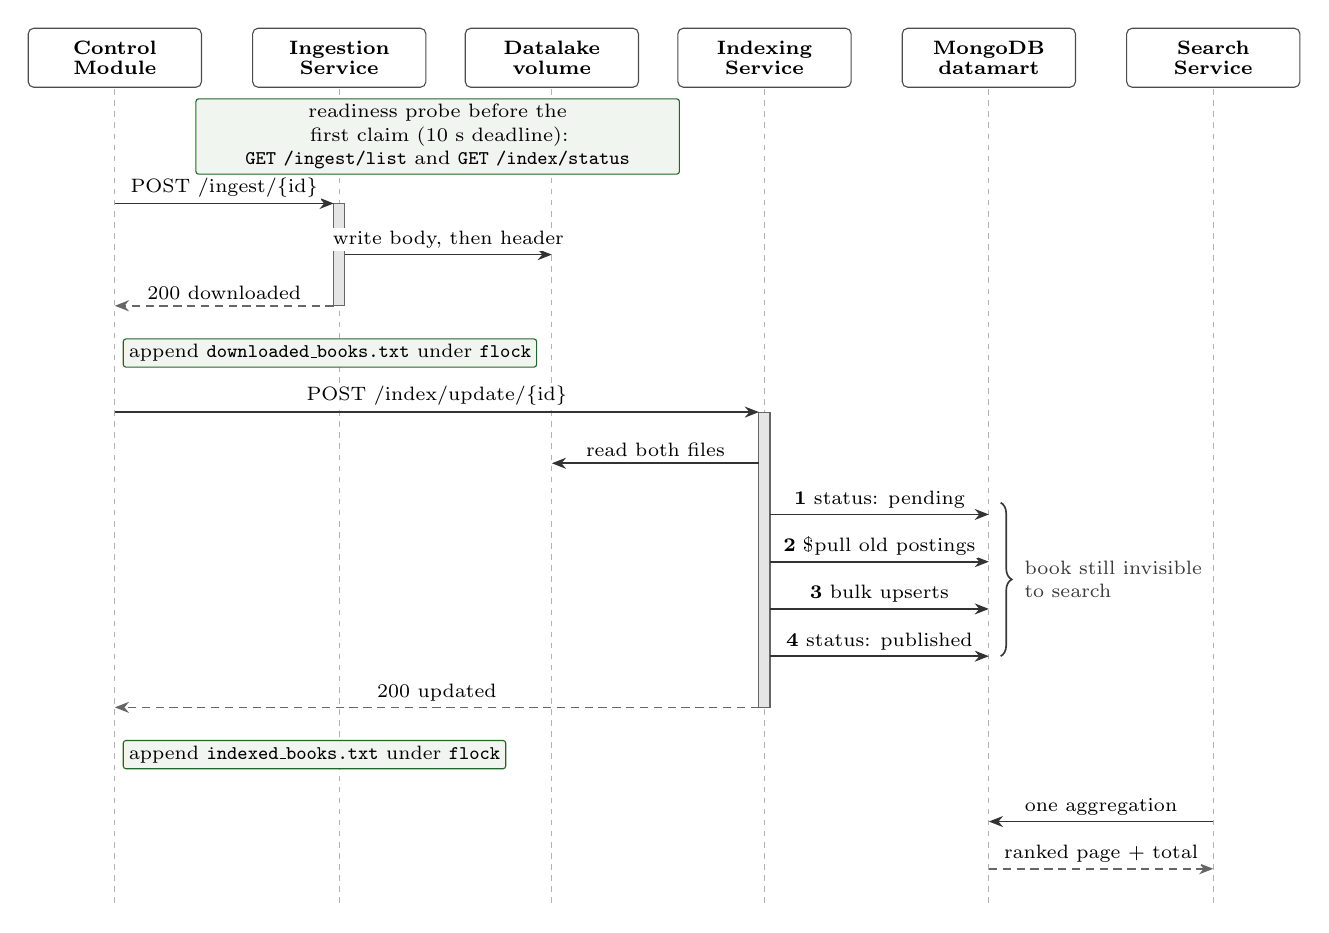
\begin{tikzpicture}[
      font=\fontsize{7}{8.4}\selectfont,
      every node/.append style={execute at begin node={\hyphenpenalty=10000\exhyphenpenalty=10000}},
      >={Stealth[length=1.8mm,width=1.4mm]},
      head/.style={draw=black!70, fill=white, rounded corners=2pt, align=center,
                   minimum width=2.2cm, minimum height=0.75cm, font=\fontsize{7}{8.4}\selectfont\bfseries},
      life/.style={draw=black!30, dash pattern=on 2pt off 2pt},
      msg/.style={->, draw=black!80, line width=0.6pt},
      ret/.style={->, draw=black!60, line width=0.6pt, dash pattern=on 3pt off 2pt},
      mlabel/.style={fill=white, inner sep=1pt, above=1pt},
      note/.style={draw=coordc!80!black, fill=zoneint, rounded corners=1pt, inner sep=2pt, align=center},
      act/.style={draw=black!60, fill=black!10},
    ]
    \def\xC{0.9} \def\xG{3.75} \def\xL{6.45} \def\xI{9.15} \def\xM{12.0} \def\xS{14.85}
    \node[head] at (\xC,0) {Control\\[-1pt]Module};
    \node[head] at (\xG,0) {Ingestion\\[-1pt]Service};
    \node[head] at (\xL,0) {Datalake\\[-1pt]volume};
    \node[head] at (\xI,0) {Indexing\\[-1pt]Service};
    \node[head] at (\xM,0) {MongoDB\\[-1pt]datamart};
    \node[head] at (\xS,0) {Search\\[-1pt]Service};
    \foreach \x in {\xC,\xG,\xL,\xI,\xM,\xS} { \draw[life] (\x,-0.4) -- (\x,-10.75); }

    \filldraw[act] (\xG-0.07,-1.85) rectangle (\xG+0.07,-3.15);
    \filldraw[act] (\xI-0.07,-4.5) rectangle (\xI+0.07,-8.25);

    \node[note, text width=6.0cm] at (5.0,-1.0)
      {readiness probe before the first claim (10 s deadline):\\
       \route{GET /ingest/list} and \route{GET /index/status}};

    \draw[msg] (\xC,-1.85) -- node[mlabel] {POST /ingest/\{id\}} (\xG-0.07,-1.85);
    \draw[msg] (\xG+0.07,-2.5) -- node[mlabel] {write body, then header} (\xL,-2.5);
    \draw[ret] (\xG-0.07,-3.15) -- node[mlabel] {200 downloaded} (\xC,-3.15);
    \node[note, anchor=west] at (\xC+0.1,-3.75) {append \code{downloaded\_books.txt} under \code{flock}};

    \draw[msg] (\xC,-4.5) -- node[mlabel] {POST /index/update/\{id\}} (\xI-0.07,-4.5);
    \draw[msg] (\xI-0.07,-5.15) -- node[mlabel] {read both files} (\xL,-5.15);
    \draw[msg] (\xI+0.07,-5.8) -- node[mlabel] {\textbf{1} status: pending} (\xM,-5.8);
    \draw[msg] (\xI+0.07,-6.4) -- node[mlabel] {\textbf{2} \$pull old postings} (\xM,-6.4);
    \draw[msg] (\xI+0.07,-7.0) -- node[mlabel] {\textbf{3} bulk upserts} (\xM,-7.0);
    \draw[msg] (\xI+0.07,-7.6) -- node[mlabel] {\textbf{4} status: published} (\xM,-7.6);
    \draw[ret] (\xI-0.07,-8.25) -- node[mlabel] {200 updated} (\xC,-8.25);
    \node[note, anchor=west] at (\xC+0.1,-8.85) {append \code{indexed\_books.txt} under \code{flock}};

    \draw[decorate, decoration={brace, amplitude=4pt}, draw=inksec!70!black, line width=0.6pt]
      (\xM+0.15,-5.65) -- (\xM+0.15,-7.6)
      node[midway, right=5pt, align=left, text=inksec!70!black]
      {book still invisible\\ to search};

    \draw[msg] (\xS,-9.7) -- node[mlabel] {one aggregation} (\xM,-9.7);
    \draw[ret] (\xM,-10.3) -- node[mlabel] {ranked page + total} (\xS,-10.3);
  \end{tikzpicture}
  \caption{Lifecycle of one book under the orchestration workflow: solid arrows
  are requests or writes, dashed arrows responses, and green notes the readiness
  probe and the completion markers of the control state. Steps 1--4 are the
  ordered datamart writes of one index update (\cref{sec:impl-indexing}); the
  book becomes visible to search only at step~4, so a crash at any earlier step
  leaves it invisible rather than half-indexed.}
  \label{fig:lifecycle}
\end{figure}

\subsection{Processes, replicas and threads}
\label{sec:replicas-threads}

The assignment distinguishes three levels of concurrency, which this report
keeps separate throughout: \emph{client concurrency} (how many requests the
front-end or the load generator keeps in flight), \emph{process replicas} (how
many instances of a service run) and \emph{threads} (how many concurrent
activities one process executes). \Cref{fig:concurrency} maps them onto the
two request paths of the system.

\begin{figure}[htbp]
  \centering
  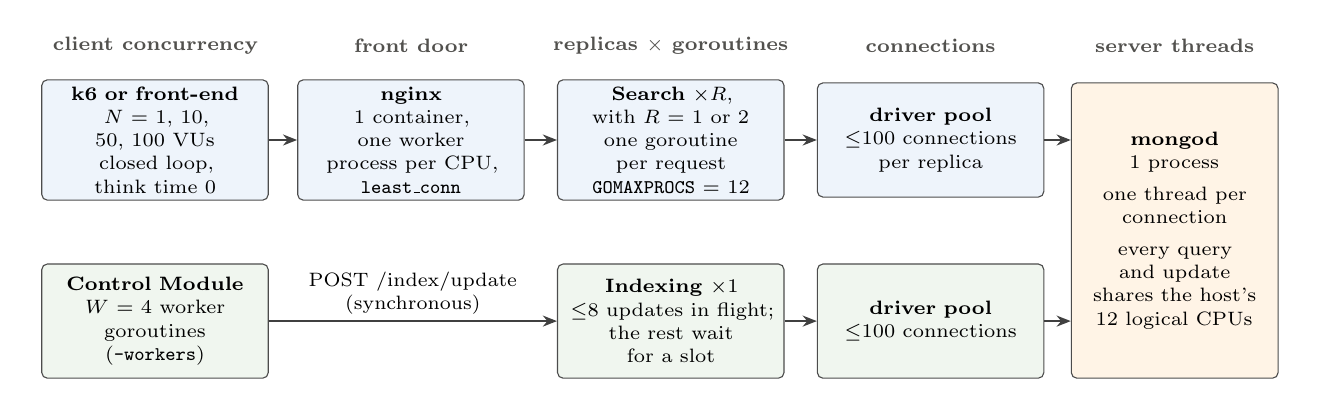
\begin{tikzpicture}[
      font=\fontsize{7}{8.4}\selectfont,
      every node/.append style={execute at begin node={\hyphenpenalty=10000\exhyphenpenalty=10000}},
      >={Stealth[length=1.8mm,width=1.4mm]},
      lvl/.style={draw=black!70, rounded corners=2pt, align=center, fill=white,
                  text width=2.7cm, minimum height=1.45cm, inner sep=2.5pt},
      arr/.style={->, draw=black!75, line width=0.7pt},
      hdr/.style={font=\fontsize{7}{8.4}\selectfont\bfseries, align=center, text width=3.0cm, text=inksec},
    ]
    \node[hdr] at (1.5,1.2) {client concurrency};
    \node[hdr] at (4.75,1.2) {front door};
    \node[hdr] at (8.05,1.2) {replicas $\times$ goroutines};
    \node[hdr] at (11.35,1.2) {connections};
    \node[hdr] at (14.45,1.2) {server threads};

    \node[lvl, fill=zonefront] (k6) at (1.5,0)
      {\textbf{k6 or front-end}\\ $N$ = 1, 10, 50, 100 VUs\\ closed loop, think time 0};
    \node[lvl, fill=zonefront] (ngx) at (4.75,0)
      {\textbf{nginx}\\ 1 container, one worker\\ process per CPU,\\ \code{least\_conn}};
    \node[lvl, fill=zonefront] (srch) at (8.05,0)
      {\textbf{Search} $\times R$, with $R$ = 1 or 2\\ one goroutine per request\\ \code{GOMAXPROCS} = 12};
    \node[lvl, fill=zonefront] (pool1) at (11.35,0)
      {\textbf{driver pool}\\ $\le$100 connections\\ per replica};

    \node[lvl, fill=zoneint] (ctl) at (1.5,-2.3)
      {\textbf{Control Module}\\ $W$ = 4 worker goroutines\\ (\code{-workers})};
    \node[lvl, fill=zoneint] (idx) at (8.05,-2.3)
      {\textbf{Indexing} $\times 1$\\ $\le$8 updates in flight;\\ the rest wait for a slot};
    \node[lvl, fill=zoneint] (pool2) at (11.35,-2.3)
      {\textbf{driver pool}\\ $\le$100 connections};

    \node[draw=black!70, rounded corners=2pt, fill=storefill, align=center, text width=2.45cm,
          minimum height=3.75cm, inner sep=2.5pt] (mongod) at (14.45,-1.15)
      {\textbf{mongod}\\ 1 process\\[3pt] one thread per\\ connection\\[3pt] every query and update\\ shares the host's\\ 12 logical CPUs};

    \draw[arr] (k6) -- (ngx);
    \draw[arr] (ngx) -- (srch);
    \draw[arr] (srch) -- (pool1);
    \draw[arr] (pool1) -- (pool1 -| mongod.west);
    \draw[arr] (ctl) -- node[above=1pt, align=center, fill=white, inner sep=1pt]
      {POST /index/update\\ (synchronous)} (idx);
    \draw[arr] (idx) -- (pool2);
    \draw[arr] (pool2) -- (pool2 -| mongod.west);
  \end{tikzpicture}
  \caption{Levels of concurrency on the read path (top) and on the indexing
  write path (bottom). Client concurrency is set by the k6 virtual users (VUs)
  or by the Control Module's workers; replication multiplies the Search
  processes behind nginx; inside every Go process, \code{net/http} serves each
  request on its own goroutine, which the runtime multiplexes onto
  \code{GOMAXPROCS} operating-system threads. Every path ends in the same
  \code{mongod} process.}
  \label{fig:concurrency}
\end{figure}

\paragraph{Distribution of requests among replicas.}
nginx re-resolves the compose service name \code{search} every 5~s and sends
each request to the replica with the fewest requests in flight
(\code{least\_conn}), so replicas can be added without restarting the proxy;
\cref{sec:decision-replicas} justifies these settings.

\paragraph{Threads inside a process.}
Every service is a Go process that serves each request on its own goroutine
(\cref{fig:concurrency}). A goroutine blocked on network input or output (a
MongoDB round trip, a Gutenberg download) is parked by the runtime and holds no
operating-system thread. Concurrency that would overload a shared resource
(downloads, index updates, Control workers) is bounded explicitly with buffered
channels used as semaphores, and shared in-process state is protected by
mutexes (\cref{sec:decision-concurrency}).

\paragraph{Concurrent access to shared storage.}
Separate processes never share memory: they share the datalake, the
control-state volume and the MongoDB server, and the rules that make their
concurrent access safe are the shared-state contracts of
\cref{tab:shared-state}.

\subsection{Shared storage}
\label{sec:storage}

\paragraph{Datalake.}
The named volume \code{datalake}, shared by the Ingestion and Indexing
services, keeps the batch-based layout selected in Stage~1: each book has a
folder \code{batch\_<low>\_<high>/\allowbreak<book\_id>/} that holds
\code{<book\_id>\_body.txt} and \code{<book\_id>\_header.txt}, with 1{,}000
consecutive IDs per batch folder, so book 1342 lives in
\code{batch\_1000\_1999/1342/}.

\paragraph{Datamart.}
The MongoDB database (\code{boogle} by default; \code{boogle\_bench} for the
benchmarks) holds three collections, described in \cref{tab:collections}. Both
services call an idempotent \code{EnsureIndexes} at start-up, so a fresh server
needs no manual set-up.

\begin{table}[htbp]
  \centering
  \small
  \caption{Collections of the MongoDB datamart.}
  \label{tab:collections}
  \begin{tabularx}{\textwidth}{@{}l>{\raggedright\arraybackslash}X>{\raggedright\arraybackslash}p{4.6cm}@{}}
    \toprule
    Collection & Document & Secondary indexes \\
    \midrule
    \code{books} & \code{\{\_id: book\_id, title, author, language,
      publication\_year, release\_year, status\}}; \code{status} is
      \code{pending} or \code{published} & \code{\{author, language,
      publication\_year\}}, \code{\{language\}}, \code{\{publication\_year\}} \\
    \code{inverted\_index} & \code{\{\_id: term, postings: [\{book\_id, tf\}]\}},
      one document per normalised term, postings sorted by \code{book\_id}
      without duplicates & \code{\{postings.book\_id\}} (multikey) \\
    \code{locks} & \code{\{\_id: "rebuild", owner, expires\_at\}}: the rebuild
      lease & --- \\
    \bottomrule
  \end{tabularx}
\end{table}

\paragraph{Control state.}
The named volume \code{control-state} holds the Control Module's three
append-only files, \code{downloaded\_books.txt}, \code{indexed\_books.txt} and
\code{failed\_books.txt}; their format and locking are specified in
\cref{tab:shared-state}.

\subsection{Single-host deployment}
\label{sec:deployment}

The whole system is described by one \code{docker-compose.yml}: the services
\code{mongo}, \code{ingestion}, \code{indexing}, \code{search} (replica count
from \code{SEARCH\_REPLICAS}) and \code{nginx}, plus the Control Module, which
is started on demand under the \code{tools} profile. One multi-stage
\code{Dockerfile} builds the four statically linked Go binaries into images
that run as an unprivileged user. Containers carry code only: the datalake,
the control state and the datamart live in named volumes, so recreating a
container never loses pipeline state. Services reach one another by compose
service name, and every port, address and data path comes from configuration
(\cref{sec:decision-deployment}). Health checks gate the start-up order: the
Indexing and Search services wait for a healthy MongoDB, nginx for a healthy
Search replica, and the Control Module for healthy Ingestion and Indexing
services.

Every process, including the MongoDB server, the reverse proxy and, during
the benchmarks, the k6 load generator and the resource sampler, runs on the
one host described in \cref{tab:host}. No container had CPU or memory limits in
the official session, so all processes competed for the same 12 logical CPUs
and 9.7~GiB of memory.

\section{API Design and Contracts}
\label{sec:api}

\subsection{Consumers and use cases}
\label{sec:use-cases}

The interfaces serve three kinds of consumer: the front-end; the Control
Module, which consumes the internal APIs (use cases UC4--UC8); and operational
components such as Docker health checks and the interactive documentation
(UC9). \Cref{tab:inventory} lists the operations of each. The front-end, a
browser application or an HTTP client such as k6 or \code{curl} exercising the
same contract during Stage~2, has three use cases:

\begin{itemize}
  \item \emph{UC1}: search books by one or more keywords, with optional author,
  language and publication-year filters and paginated results;
  \item \emph{UC2}: open the detail page of one book;
  \item \emph{UC3}: populate the filter controls with the values that actually
  occur in the catalogue.
\end{itemize}

The front-end never reads files, never connects to MongoDB and does not need
to know how the services are coordinated: its contract describes application
data only, and ingestion commands, index rebuilds and datalake paths do not
appear in it.

\subsection{Endpoint inventory}
\label{sec:inventory}

\Cref{tab:inventory} is the consolidated inventory, grouped by consumer. Every
operation is \emph{synchronous}: the response is sent when the work has
completed (or failed), never when it has merely been accepted. Every operation
is also \emph{idempotent}, so a caller may repeat it after a timeout without
creating duplicates. Both properties are stated per operation in the
specification through the vendor extensions \code{x-completion} and
\code{x-idempotent}.

\begin{table}[htbp]
  \centering
  \footnotesize
  \caption{Endpoint inventory. Front-end routes are published by nginx on port
  7003; internal routes are served on ports 7001 (Ingestion) and 7002
  (Indexing). Error codes and their meaning are listed in \cref{tab:errors}.}
  \label{tab:inventory}
  \renewcommand{\arraystretch}{1.12}
  \begin{tabularx}{\textwidth}{@{}>{\raggedright\arraybackslash}p{3.95cm}>{\raggedright\arraybackslash}p{2.3cm}>{\raggedright\arraybackslash}X>{\raggedright\arraybackslash}p{2.3cm}@{}}
    \toprule
    Method and route & Provider $\rightarrow$ consumer & Purpose & Status codes \\
    \midrule
    \multicolumn{4}{@{}l}{\textbf{Front-end-facing} (public, through nginx :7003)} \\
    \route{GET /search} & Search $\rightarrow$ front-end & UC1: keyword search with
      optional filters, ranking and pagination & 200, 400, 500 \\
    \route{GET /books/\allowbreak\{book\_id\}} & Search $\rightarrow$ front-end & UC2: metadata
      of one published book & 200, 400, 404, 500 \\
    \route{GET /search/filters} & Search $\rightarrow$ front-end & UC3: distinct
      languages and publication years of published books & 200, 500 \\
    \route{OPTIONS} (any route) & Search $\rightarrow$ browser & CORS preflight of a
      cross-origin page & 204, 403 \\
    \midrule
    \multicolumn{4}{@{}l}{\textbf{Internal} (consumer: Control Module)} \\
    \route{POST /ingest/\allowbreak\{book\_id\}} & Ingestion $\rightarrow$ Control & UC4:
      download, split and store one book & 200, 400, 404, 500, 503 \\
    \route{GET /ingest/status/\allowbreak\{book\_id\}} & Ingestion $\rightarrow$ Control &
      UC5: is the book complete in the datalake? & 200, 400, 404 \\
    \route{GET /ingest/list} & Ingestion $\rightarrow$ Control & UC6: complete
      books, in ascending order (\code{-discover}) & 200, 500 \\
    \route{POST /index/update/\allowbreak\{book\_id\}} & Indexing $\rightarrow$ Control & UC7:
      index one book and publish it & 200, 400, 404, 500 \\
    \route{POST /index/rebuild} & Indexing $\rightarrow$ Control (admin.) & UC8:
      rebuild the datamart from the whole datalake & 200, 409, 500, 503 \\
    \midrule
    \multicolumn{4}{@{}l}{\textbf{Operational}} \\
    \route{GET /index/status} & Indexing $\rightarrow$ Control, k6, Docker &
      Indexing statistics; readiness probe; corpus guard of the search benchmark
      & 200 \\
    Health checks & every service $\rightarrow$ Docker & \route{GET /ingest/list},
      \route{GET /index/status}, \route{GET /search/filters} (replicas and nginx),
      \code{mongosh} ping & 200 \\
    \route{GET /books/\allowbreak\{book\_id\}} & Search $\rightarrow$ Control & \code{-verify}
      mode: reconcile \code{indexed\_books.txt} with the datamart & 200, 404 \\
    \route{GET /swagger/index.html} & every service $\rightarrow$ developers &
      UC9: interactive OpenAPI documentation (\code{/swagger/doc.json}) & 200 \\
    \bottomrule
  \end{tabularx}
\end{table}

\subsection{Front-end contract}
\label{sec:frontend-contract}

\paragraph{GET /search.}
The required search operation and all its filter combinations are variants of
this single endpoint. \Cref{tab:search-params} specifies its parameters.
Several design rules complete the contract.

\begin{itemize}
  \item \textbf{Term semantics.} \code{q} is split exactly like book text:
  runs of the letters a--z, case-insensitive, so digits, spaces and punctuation
  separate words (\code{Moby-Dick} searches \code{moby} AND \code{dick}).
  Repeated words count once. Stop words (\emph{the}, \emph{and}, \emph{of},
  \ldots), single letters and Roman numerals are never indexed and are
  ignored, so a \code{q} made only of them matches nothing and returns 200 with
  an empty page. A book matches only if it contains \emph{every} remaining
  term (AND). The Search Service reuses the Indexing Service's tokenizer, so a
  query word and a body word always normalise alike.
  \item \textbf{Filters} combine with AND. \code{author} is a case-insensitive
  substring match, \code{language} an exact, case-insensitive ISO~639 code that
  matches any code of a multilingual book (stored as \code{"en,fr"}), and
  \code{year} an exact \code{publication\_year}. Empty filter values are treated
  as absent, and only applied filters are echoed in \code{filters}.
  \item \textbf{Ordering.} Results are ranked by relevance, defined as the sum
  of the query terms' frequencies in the book, in descending order, with ties
  broken by ascending \code{book\_id}, so pagination is deterministic.
  \item \textbf{Pagination.} \code{total} counts every match across all pages,
  whereas \code{results} holds at most \code{limit} books starting at
  \code{offset}. A valid query without matches, or an \code{offset} past the
  last match, returns 200 with \code{results: []} and the true \code{total}.
  \item \textbf{Limits.} At most 10 distinct terms per query and 100 results
  per page are accepted.
\end{itemize}

\begin{table}[htbp]
  \centering
  \footnotesize
  \caption{Parameters of \route{GET /search}. Violations are answered with
  \code{400 invalid\_parameter} (or \code{missing\_parameter} for an absent
  \code{q}) and a message naming the parameter.}
  \label{tab:search-params}
  \begin{tabularx}{\textwidth}{@{}llll>{\raggedright\arraybackslash}X@{}}
    \toprule
    Parameter & Type & Required & Default & Validation and semantics \\
    \midrule
    \code{q} & string & yes & --- & At least one word of letters a--z and at
      most 10 distinct terms; AND of its terms \\
    \code{author} & string & no & none & Case-insensitive substring of the author \\
    \code{language} & string & no & none & ISO~639 code, case-insensitive, any code
      of the book \\
    \code{year} & integer & no & none & 1--9999; exact publication year \\
    \code{offset} & integer & no & 0 & 0--$2^{31}-1$; matches skipped before the page \\
    \code{limit} & integer & no & 20 & 1--100; maximum results in the page \\
    \bottomrule
  \end{tabularx}
\end{table}

A representative exchange, taken verbatim from the validation transcript
(check S5 in \cref{tab:validation}), shows the response schema:

\begin{lstlisting}
GET /search?q=adventure&author=austen&language=en&limit=5          -> 200 OK
{"query":"adventure","filters":{"author":"austen","language":"en"},
 "total":1,"offset":0,"limit":5,
 "results":[{"book_id":1342,"title":"Pride and Prejudice",
             "author":"Jane Austen","language":"en","year":0}]}
\end{lstlisting}

\paragraph{GET /books/\allowbreak\{book\_id\} and GET /search/filters.}
These two routes serve UC2 and UC3. \route{GET /books/\allowbreak\{book\_id\}}
returns the same record as one search result, and only for a \emph{published}
book: a book still being indexed is as invisible here as in search.
\route{GET /search/filters} returns \code{\{"languages": [...], "years":
[...]\}}, computed from published books only.

\subsection{Internal contracts}
\label{sec:internal-contracts}

\paragraph{Ingestion.}
\route{POST /ingest/\allowbreak\{book\_id\}} answers \code{downloaded} once both
files are stored, or \code{available} without downloading when the book was
already complete; a failure is either permanent (\code{404}) or transient
(\code{503}), as listed in \cref{tab:errors}. Concurrent requests for the same
book join one shared download, so the endpoint is safe under duplicate
submissions.

\paragraph{Indexing.}
\route{POST /index/update/\allowbreak\{book\_id\}} answers \code{updated} once the
book's metadata and postings are in the \emph{published} index, visible to every
request that starts afterwards. Re-indexing replaces the book's metadata and
postings, including terms the new version no longer contains, so repeating the
call leaves the index exactly as after the first one; an update that arrives
during a rebuild is not blocked but replayed on the rebuilt index.
\route{POST /index/rebuild} builds a new catalogue and index aside and
publishes them in one step, so search keeps reading the previous complete
index until the swap, and also when the rebuild fails (\cref{tab:errors}).
\route{GET /index/status}
reports the published books, the time of the last change and the document
bytes of the datamart (\code{dbStats.dataSize}). The literal request and
response bodies of every internal operation are recorded in
\code{docs/api\_inventory.md} and the service specifications under \code{api/}.

\paragraph{Timeouts and retries expected of the caller.}
The specification states, per operation, the timeout and failure behaviour
expected of the caller, which the Control Module implements
(\cref{sec:impl-control}). A call to
\route{POST /ingest} may take up to 150~s, above the service's own 2-minute
budget, so the service always answers before the caller gives up. Indexing,
status and readiness calls are bounded at 30~s. Transient failures (transport
errors, timeouts, \code{408}, \code{429}, \code{5xx}) are retried three times
with a doubling backoff that starts at 1~s, while permanent ones (other
\code{4xx}) are recorded once and not retried. A client that disconnects
cancels only its own index update, because the request context is propagated
down to the MongoDB writes, whereas a shared download continues for the other
callers that joined it.

\subsection{Error model and status codes}
\label{sec:errors}

Every service answers errors with the same JSON body,
\code{\{"error": "<code>", "message": "<human-readable explanation>"\}}, where
\code{error} is a stable machine-readable code and \code{message} is meant for
logs and developers; \cref{tab:errors} lists every code.

\begin{table}[htbp]
  \centering
  \footnotesize
  \caption{Error codes shared by the three APIs.}
  \label{tab:errors}
  \begin{tabularx}{\textwidth}{@{}lc>{\raggedright\arraybackslash}p{4.3cm}>{\raggedright\arraybackslash}X@{}}
    \toprule
    Code & HTTP & Raised by & Meaning and expected caller action \\
    \midrule
    \code{missing\_parameter} & 400 & \route{GET /search} & \code{q} is absent; fix the request \\
    \code{invalid\_parameter} & 400 & \route{GET /search} & \code{q} has no word or more than 10
      distinct terms, or \code{year}, \code{offset}, \code{limit} out of range \\
    \code{invalid\_book\_id} & 400 & every \code{\{book\_id\}} route & Path parameter is not a positive integer \\
    \code{book\_not\_found} & 404 & \route{GET /books}, \route{GET /ingest/status},
      \route{POST /index/update} & No published book (search) or no complete
      datalake copy (internal); ingest first, then retry \\
    \code{book\_unavailable} & 404 & \route{POST /ingest} & Gutenberg has no such
      book or no START/END markers; permanent, record the failure \\
    \code{origin\_not\_allowed} & 403 & CORS preflight & Origin outside
      \code{CORS\_ALLOWED\_ORIGIN} \\
    \code{rebuild\_in\_progress} & 409 & \route{POST /index/rebuild} & Another
      replica holds the lease; poll \route{GET /index/status} instead \\
    \code{internal\_error} & 500 & any & Storage failure; retry with backoff \\
    \code{download\_failed} & 503 & \route{POST /ingest} & Transient Gutenberg
      failure or budget exhausted; retry with backoff \\
    \code{rebuild\_interrupted} & 503 & \route{POST /index/rebuild} & Budget ran
      out or caller left; previous index still published; retry later \\
    \bottomrule
  \end{tabularx}
\end{table}

\subsection{Non-HTTP contracts: shared state}
\label{sec:shared-state-contracts}

Not every interaction is an HTTP call. The coordination of
\cref{sec:coordination} also relies on shared state whose layout, ownership and
synchronisation rules form part of the contract (\cref{tab:shared-state}).
They agree with \cref{fig:architecture,fig:lifecycle}.

\begin{table}[htbp]
  \centering
  \footnotesize
  \caption{Shared-state contracts: what each record means, who may write it and
  how concurrent access is synchronised.}
  \label{tab:shared-state}
  \begin{tabularx}{\textwidth}{@{}>{\raggedright\arraybackslash}p{2.5cm}>{\raggedright\arraybackslash}p{2.2cm}>{\raggedright\arraybackslash}p{2.35cm}>{\raggedright\arraybackslash}p{3.4cm}>{\raggedright\arraybackslash}X@{}}
    \toprule
    Contract & Location & Writer / readers & Synchronisation & Semantics \\
    \midrule
    Datalake completeness & datalake volume & Ingestion / Ingestion, Indexing &
      Atomic replace per file (temporary file, \code{fsync}, rename); body
      before header & A book exists for readers if and only if both files exist \\
    Control-state files & control-state volume & Control Module only &
      Exclusive \code{flock} to append, shared \code{flock} to read & One book ID
      per line; \code{failed\_books.txt} holds \code{<id><TAB><reason>} \\
    Publication state & \code{books.status} & Indexing / Search & Atomic
      per-document update; ordered writes (\cref{fig:lifecycle}) & Search returns
      \code{published} books only \\
    Rebuild lease & \code{locks}, \code{\_id: "rebuild"} & Indexing replicas &
      Claimed with \code{findOneAndUpdate}; 2-minute expiry, renewed every 30~s;
      taken over once expired & One rebuild at a time across replicas; the
      loser gets 409 \\
    Rebuild publication & \code{*\_rebuild} collections & Lease holder / Search &
      \code{renameCollection} with \code{dropTarget}, index first, then books &
      Readers see the old or the new complete datamart \\
    \bottomrule
  \end{tabularx}
\end{table}

\subsection{Exposure and cross-origin access}
\label{sec:cors}

The front-end reaches the Search API through one entry point, nginx on port
7003, whatever the number of replicas. For a browser page served from another
origin, the Search Service applies CORS to every route: the allowed origins
come from \code{CORS\_ALLOWED\_ORIGIN} (\code{*} by default, safe for a
read-only API without credentials, or an explicit list), and a preflight is
answered with \code{204} or \code{403} (check X4 in \cref{tab:validation}).
The internal ports 7001 and 7002 are also published on the host, for the
Control Module and the Swagger pages, but the front-end contract never uses
them.

\subsection{Specification and validation evidence}
\label{sec:validation}

\paragraph{Versioned specification.}
Each service carries a versioned OpenAPI~2.0 (Swagger) document, version
1.0.0, under \code{api/ingestion/}, \code{api/indexing/} and \code{api/search/}
(\code{swagger.yaml} and \code{swagger.json}), published with the code at
\url{\repourl/tree/develop/api}. The documents are generated with
\code{swaggo/swag} v1.16.6 from annotations next to the handlers
(\cref{sec:decision-api}), and each running service serves its own document as
an interactive page at \route{/swagger/index.html}. Beyond schemas,
parameters, defaults and status codes, every operation records its provider,
consumers and audience (\code{x-provider}, \code{x-consumers},
\code{x-audience}), the completion and idempotency extensions of
\cref{sec:inventory}, and the timeouts and retries expected of the caller.

\paragraph{API validation script (19/19).}
\code{scripts/api\_validation.sh} is the runnable check of the front-end
contract. It seeds four fixture books (82, 84, 1341 and 1342) through the
stack's own \route{POST /ingest} and \route{POST /index/update} routes, which
exercises the internal contracts on the way, then sends nineteen requests to
nginx on port 7003 and asserts status codes, error codes and response
invariants that depend only on the fixtures, never on corpus-dependent totals.
It exits with status~1 on any failure, so it doubles as a regression test, and
\code{--record} regenerates
\code{docs/evidence/\allowbreak api\_validation\_results.md} with the literal
response body of every check. The recorded run of 31~October~2026 passed
\textbf{19 of 19} checks (\cref{tab:validation}).

\begin{table}[htbp]
  \centering
  \footnotesize
  \caption{The 19 checks of \code{scripts/api\_validation.sh} and their recorded
  outcome (\code{docs/evidence/\allowbreak api\_validation\_results.md}). Every check passed.}
  \label{tab:validation}
  \begin{tabularx}{\textwidth}{@{}l>{\raggedright\arraybackslash}p{3.3cm}>{\raggedright\arraybackslash}p{5.2cm}>{\raggedright\arraybackslash}X@{}}
    \toprule
    ID & Case & Request & Expected (and observed) \\
    \midrule
    S1 & Keyword search & \route{/search?q=frankenstein} & 200; book 84 present \\
    S2 & Author filter & \route{q=adventure\&author=Austen} & 200; 1342 present; every author contains ``austen'' \\
    S3 & Language filter & \route{q=adventure\&language=EN} & 200; filter echoed as \code{en}; every result in \code{en} \\
    S4 & Year filter & \route{q=adventure\&year=1818} & 200; filter echoed; no result breaks it \\
    S5 & Combined filters & \route{q=adventure\&author=austen\&\allowbreak language=en\&limit=5} & 200; 1342 present; 82 and 84 absent \\
    S6 & No matches & \route{q=quidditch} & 200; \code{total} 0; \code{results} [] \\
    S7 & Offset past the end & \route{q=adventure\&offset=1000000} & 200; \code{results} []; \code{total} still 3 \\
    V1 & Missing \code{q} & \route{/search} & 400 \code{missing\_parameter} \\
    V2 & \code{limit}=0 & \route{q=adventure\&limit=0} & 400 \code{invalid\_parameter} naming \code{limit} \\
    V3 & \code{limit}=101 & \route{q=adventure\&limit=101} & 400 \code{invalid\_parameter} naming \code{limit} \\
    V4 & \code{year}=abc & \route{q=adventure\&year=abc} & 400 \code{invalid\_parameter} naming \code{year} \\
    B1 & Book by ID & \route{/books/84} & 200; metadata of book 84 \\
    B2 & Unknown book & \route{/books/99999999} & 404 \code{book\_not\_found} \\
    B3 & Malformed ID & \route{/books/abc} & 400 \code{invalid\_book\_id} \\
    F1 & Filter values & \route{/search/filters} & 200; \code{languages} includes \code{en}; \code{years} is an array \\
    X1 & Multi-word AND & \route{q=modern+prometheus} & 200; only book 84 \\
    X2 & No word in \code{q} & \route{q=1813} & 400 \code{invalid\_parameter} naming \code{q} \\
    X3 & Stop words only & \route{q=the} & 200; \code{total} 0 \\
    X4 & CORS preflight & \route{OPTIONS /search?q=whale} from \code{localhost:5173} & 204 with \code{Access-Control-Allow-Origin} \\
    \bottomrule
  \end{tabularx}
\end{table}

The run used local processes and MongoDB~8.3.7 at commit \code{c2cb456},
which predates the fallback of \code{publication\_year} to the release year, so
check S4 verified the \emph{contract} of the year filter (applied, echoed,
never violated) on fixtures without a known year (\cref{sec:validity}).

\paragraph{Internal interactions and further evidence.}
The internal HTTP contracts are exercised end to end by two scripts whose
transcripts are committed. \code{scripts/e2e\_control.sh} checks
orchestration of real Gutenberg books, restart semantics (a replayed run skips
finished books and leaves the state files intact), permanent-failure recording
and discovery mode. \code{scripts/e2e\_compose.sh} checks the Docker deployment
in eight steps: health of every container, orchestration, idempotent replay,
the front-facing routes, the fail-fast refusal of the Control Module while
ingestion is down, recovery after relaunch, persistence of datalake and
datamart across container recreation, and teardown; all pass. The
cross-replica rebuild lease was verified live
(\code{docs/evidence/\allowbreak rebuild\_replica.md}, \cref{sec:bench-indexing}). Under
load, the k6 checks \emph{page respects limit} and \emph{pagination is echoed}
held for 100\% of the 65{,}950 successful queries of the two search runs. The
unit and integration tests are summarised in \cref{sec:testing}.

\section{Microservice Implementation}
\label{sec:implementation}

\subsection{Technology stack and code organisation}
\label{sec:stack}

The assignment's reference template is a Java~17 service built with Javalin,
Gson and Maven and benchmarked with JMH. The group implemented the services in
\textbf{Go} instead, the language selected by the Stage~1 measurements
(highest datalake write throughput of the four implementations compared, and
fastest index builds from 500 books upward), and every element of the template
has a standard counterpart. The \code{net/http} server with the method-aware
\code{http.ServeMux} of Go~1.22, which answers \code{405} to an undeclared
method, replaces Javalin without any third-party framework;
\code{encoding/json}, with struct tags that fix the field names of the
contract, replaces Gson; one Go module (\code{boogle-engine}, Go~1.25) with
four entry points under \code{cmd/} replaces Maven; and \code{testing.B} with
\code{benchstat} replaces JMH, with the benchmarks kept in \code{\_test.go}
files and therefore out of the service binaries. The datamart is accessed
through the official MongoDB Go driver (v2.9.2), the API documentation is
generated with \code{swaggo/swag}, and logging uses the structured
\code{log/slog} logger.

\paragraph{Repository layout.}
The Go code follows a \textbf{hexagonal (ports and adapters) structure}: each
use case lives in a \emph{core} package that declares, as Go interfaces, the
operations it offers (\emph{driving} ports such as \code{Searcher}) and the
operations it needs (\emph{driven} ports such as \code{search.Index}). Source
dependencies point only into the core, and every adapter asserts at compile
time the ports it implements, so the use cases are tested with in-memory fakes
and moving a store to Stage~3 infrastructure means writing a new adapter rather
than changing a service. The packages are grouped as follows (the full table is
in \code{docs/architecture.md}):

\begin{itemize}
  \item \emph{Cores} (no HTTP, MongoDB or filesystem code): \code{internal/models}
    (domain and shared errors), \code{internal/indexer} (tokenizer and metadata
    parser), and the use cases in \code{internal/ingestion},
    \code{internal/indexing}, \code{internal/search} and
    \code{internal/control}.
  \item \emph{Driving adapters} (inbound HTTP): \code{internal/api} (shared
    kit) and the three service packages under it (\code{ingestionapi},
    \code{indexingapi}, \code{searchapi}) with their handlers, DTOs and CORS.
  \item \emph{Driven adapters} (outbound): \code{internal/crawler},
    \code{internal/datalake}, \code{internal/mongodb},
    \code{internal/control/httpclient} and \code{internal/localstate} (the
    \code{flock}-protected state files).
  \item \emph{Composition roots, specifications and deployment}: \code{cmd/*},
    \code{api/*}, \code{deploy/nginx}, \code{docker-compose*.yml},
    \code{test/load}, \code{scripts} and \code{docs}.
\end{itemize}

The services share one skeleton: \code{main}, the composition root, parses
flags and environment variables, builds the adapters and injects them into the
core constructors (constructor injection), mounts the handlers on a
\code{ServeMux}, starts an \code{http.Server} whose read, header, write and
idle timeouts are bounded, and shuts down gracefully on \code{SIGINT} or
\code{SIGTERM} (30~s grace for Ingestion and Indexing, 10~s for Search).

\subsection{Ingestion Service}
\label{sec:impl-ingestion}

A request for \route{POST /ingest/\allowbreak\{book\_id\}} flows from the handler into
the \textbf{ingestion core} (\code{ingestion.Service}) and from there to two
driven adapters. The core implements single-flight per book: concurrent
requests for the same ID join one shared ingestion, tracked in an in-flight map
guarded by a mutex. Each ingestion runs detached from the requests that wait
for it, under its own time budget, so a caller that disconnects cancels neither
the shared work nor the other callers. If the datalake already holds the
complete book, the core returns at once; otherwise it waits for a download slot
(a buffered channel) and the \textbf{Gutenberg client} downloads
\code{https://www.gutenberg.org/\allowbreak cache/epub/<id>/pg<id>.txt} through one shared
\code{http.Client} with connection reuse, retrying only the errors it
classifies as transient. The \textbf{splitter} then separates header and body
at the START/END markers, and the \textbf{datalake} adapter stores both files
with the atomic protocol of \cref{tab:shared-state}, so a crash at any point
leaves at most a stray temporary file, never a truncated book. The budget, slot
count and retry settings are listed in \cref{tab:replicas}.

\subsection{Indexing Service}
\label{sec:impl-indexing}

\paragraph{One update.}
\route{POST /index/update/\allowbreak\{book\_id\}} first acquires an update slot
(\cref{tab:replicas}); a request that finds them all busy waits until a slot
frees or its caller disconnects, so a burst of updates cannot exhaust the
datamart connection pool. The \textbf{indexing core} (\code{indexing.Service})
then reads the book from the datalake through its \code{BookSource} port,
refusing an incomplete one, extracts the metadata from the header (title,
author, language mapped to ISO~639 codes, original publication year falling
back to the Gutenberg release year), and turns the body into terms with the
Stage~1 tokenizer, whose rules are those of the search contract
(\cref{sec:frontend-contract}). The MongoDB writer,
which implements the core's \code{IndexWriter} port, stores the book in four
ordered, idempotent steps (\cref{fig:lifecycle}):

\begin{enumerate}
  \item replace the book's metadata record with \code{status: pending};
  \item remove the book from every posting list it appeared in
  (\code{\$pull}, bounded by the multikey index on \code{postings.book\_id}),
  so a re-indexed book forgets terms it no longer contains;
  \item upsert one posting per distinct term in unordered bulk writes of at
  most 1{,}000 operations. Each upsert is an update pipeline that filters out
  any previous entry of the book (\code{\$filter}), appends the fresh
  \code{\{book\_id, tf\}} pair (\code{\$setUnion}) and re-sorts the list by
  book ID (\code{\$sortArray}), so replays converge to the same document;
  \item set \code{status: published}, the moment the book becomes searchable.
\end{enumerate}

\paragraph{Rebuild and publication.}
\route{POST /index/rebuild} first claims the cross-replica lease of
\cref{tab:shared-state}, which a background goroutine renews while the rebuild
runs. The holder streams the datalake one book at a time into the temporary
collections \code{books\_rebuild} and \code{inverted\_index\_rebuild}, so its
memory does not grow with the datalake, creates their indexes, and publishes
them with two \code{renameCollection} commands (index first, then books);
search keeps reading the previous complete datamart until the swap. Updates that
arrive during a rebuild are not blocked: an atomic flag, read \emph{before}
each datamart write, makes the indexing core record the book in a
mutex-protected replay list, and the list is re-applied to the fresh datamart after the swap,
so no concurrent update is lost. Recording before writing guarantees that a
swap can never overtake a book that is still being written.

\paragraph{Status.}
\route{GET /index/status} counts the published books and reads the datamart
size from \code{dbStats}. It never fails: a measurement that cannot be taken
is reported as zero and logged, because the endpoint doubles as a readiness
probe.

\subsection{Search Service}
\label{sec:impl-search}

The handler reads the query string and passes it to the \textbf{search core}
(\code{search.Service}), which validates it (\cref{tab:search-params}) and
splits \code{q} into at most ten distinct normalised terms with the indexer's
tokenizer. When every word of \code{q} is one the index never stores, the core
answers an empty page without querying MongoDB. Otherwise it calls its
\code{Index} port, which the MongoDB adapter implements with \textbf{one
aggregation} on \code{inverted\_index}, so a request costs a single round trip
(keeping matching and ranking in the aggregation is a deliberate choice,
discussed in \cref{sec:decision-storage}):

\begin{enumerate}
  \item \code{\$match} the term documents (\code{\_id \$in} terms) and
  \code{\$unwind} their postings;
  \item \code{\$group} the postings by book, collecting the matched terms and
  summing their frequencies into a score, then keep only the books that
  matched every term (the AND);
  \item \code{\$lookup} each surviving book in \code{books}, requiring
  \code{status: published} and applying the author, language and year filters
  inside the lookup;
  \item \code{\$facet} into a total count and a page sorted by score
  (descending) and book ID (ascending), with \code{\$skip} and \code{\$limit}.
\end{enumerate}

Intersecting the postings before the join means that every additional term
shrinks the join instead of growing it. \route{GET /books/\{id\}} and
\route{GET /search/filters} go through the catalog use case
(\code{search.CatalogService}) and read the same datamart through the same
stateless reader, restricted to published books. The process holds no mutable state
beyond the driver's connection pool, which is why replicas are interchangeable
and why nginx may route any request to any of them. At start-up the service
refuses to run if MongoDB is unreachable (fail fast), instead of answering
\code{500} to every request.

\subsection{Control Module}
\label{sec:impl-control}

The Control Module is a command-line tool (\code{cmd/control}) that selects
candidate books (\code{-ids}, \code{-from}/\code{-to}, or \code{-discover}
from \route{GET /ingest/list}), loads the control state, and refuses to start
unless both services answer their readiness routes within 10~s. A pool of
\code{-workers} goroutines (4 by default) then processes the candidates. A
mutex-protected \textbf{book selector} hands each candidate to exactly one
worker; the worker skips books already indexed or failed, ensures ingestion,
records it, ensures indexing and records it, applying the retry policy of
\cref{sec:internal-contracts} to each step. A book interrupted by
\code{SIGINT} or \code{SIGTERM} is left pending and claimed again by the next
run. Two further modes support operations:
\code{-retry-failed} atomically empties \code{failed\_books.txt} and
re-enqueues its books, and \code{-verify} reconciles \code{indexed\_books.txt}
with the datamart through \route{GET /books/\{id\}}. Every finished step is
logged with its duration, and the run summary reports throughput and the time
spent in ingestion and indexing steps, which provides the coordination-cost
measurements of \cref{sec:bench-coordination}.

\subsection{Readiness, task ownership, retries, idempotency and publication}
\label{sec:readiness}

\Cref{tab:mechanisms} gathers, for each concern the assignment names, the
mechanism that implements it.

\begin{table}[htbp]
  \centering
  \footnotesize
  \caption{How the implementation handles readiness, ownership, retries,
  idempotency and publication.}
  \label{tab:mechanisms}
  \begin{tabularx}{\textwidth}{@{}>{\raggedright\arraybackslash}p{2.75cm}>{\raggedright\arraybackslash}X>{\raggedright\arraybackslash}p{3.5cm}@{}}
    \toprule
    Concern & Mechanism & Where \\
    \midrule
    Book ready for indexing & Datalake completeness contract
      (\cref{tab:shared-state}); an incomplete book is refused &
      \code{internal/datalake}, indexing handler \\
    Service readiness & Docker health checks gate start-up; Control readiness
      probe (10~s); Indexing and Search refuse to start without MongoDB &
      \code{docker-compose.yml}, \code{cmd/*} \\
    Task ownership & Selector gives each book to one worker per run; one
      Control instance at a time; single-flight per book in Ingestion; rebuild
      lease across replicas & \code{internal/control},
      \code{internal/ingestion}, \code{rebuild\_lock.go} \\
    Retries & Control: 3 attempts with 1~s doubling backoff for transient
      failures only (\cref{sec:internal-contracts}); Ingestion downloads: same
      policy &
      \code{orchestrator.go}, \code{internal/ingestion} \\
    Idempotency & Ingestion answers \code{available} for complete books;
      index updates replace metadata and converge postings; control records
      skip known IDs & \code{ingestion}, \code{mongodb}, \code{control} \\
    Publication & \code{status: published} is the last write of an update;
      rebuild swaps complete collections; updates during a rebuild are replayed
      & \code{book\_indexer.go}, \code{rebuild.go} \\
    Crash between step and record & Book not recorded, so the next run replays
      the idempotent call & \code{orchestrator.go} \\
    \bottomrule
  \end{tabularx}
\end{table}

\subsection{Testing}
\label{sec:testing}

The repository contains unit tests for every package and integration tests that
run against a live MongoDB server. These tests skip quickly when no server is
reachable, and a recorded run of \code{go test -count=1 -v ./...} against the
\code{mongo:7} container reported 365 passing tests, none skipped and none
failing (\code{docs/evidence/\allowbreak tests.txt}). The suites cover the orchestration loop
against fake services (happy path, resumption, retries, permanent failures,
shutdown, concurrent workers), the HTTP clients against \code{httptest}
servers, every handler's contract including error codes and CORS, the write
path's idempotency and the visibility of pending books, the rebuild and its
lease, and the search aggregation's ranking, filters and pagination. The
micro-benchmarks of \cref{sec:bench-threads} live in the same
\code{\_test.go} files.

\section{Design Decisions}
\label{sec:design}

\subsection{Coordination mechanism}
\label{sec:decision-coordination}

The assignment admits four coordination strategies. \Cref{tab:coordination}
compares them against the requirements that matter for this pipeline: a book
must be indexed only after its ingestion has completed, an update must be
published before search can see it, and repeated work must not corrupt the
datamart.

\begin{table}[htbp]
  \centering
  \footnotesize
  \caption{Coordination strategies considered. The chosen design is classical
  orchestration, combined with persistent markers, a publication state and a
  lease kept in shared storage.}
  \label{tab:coordination}
  \begin{tabularx}{\textwidth}{@{}>{\raggedright\arraybackslash}p{2.3cm}>{\raggedright\arraybackslash}X>{\raggedright\arraybackslash}X>{\raggedright\arraybackslash}X>{\raggedright\arraybackslash}X@{}}
    \toprule
    Criterion & \textbf{Classical orchestration} (chosen) & Choreography with a
      broker & Time-based coordination & Shared memory \\
    \midrule
    Ingest-before-index & Explicit: indexing is called only after a
      \code{2xx} from ingestion & Implicit: a \code{BookDownloaded} event
      triggers indexing & Requires readiness markers; a fixed delay proves
      nothing & Atomic state transitions in a shared region \\
    Completion signal & Synchronous response: \code{200} means done &
      Acknowledgements, at-least-once delivery & Persistent markers, polled &
      Flags guarded by inter-process locks \\
    Extra components & None beyond a command-line tool & A broker process with
      queues and dead-letter handling & A scheduler; overlap and missed-run
      handling & Memory-mapped region, inter-process synchronisation \\
    Failure handling & One retry policy; durable progress records & Redelivery,
      duplicate suppression, ordering rules & Late or overlapping runs & Recovery
      of a region left locked by a crashed process \\
    Observability & One log with per-step durations & Requires distributed
      tracing & Run history & Hard to inspect \\
    Stage 3 & HTTP works across machines; the control state must move to
      shared storage & Natural fit for a cluster & Works with distributed markers
      & Must be replaced: single host only \\
    \bottomrule
  \end{tabularx}
\end{table}

\paragraph{Decision and rationale.}
Classical orchestration makes the one hard dependency of the pipeline explicit
in code rather than emergent from message timing, and its synchronous answers
give the clearest definition of ``done'': a book is recorded as indexed only
after it has been \emph{published}. The alternatives buy nothing on one host. A
broker would add a stateful process on a host whose CPU is already the scarce
resource (\cref{sec:bench-resources}), while still requiring the idempotent
consumers our services already are; time-based runs would only add latency on
top of the readiness markers needed anyway; and shared memory is unsafe across
containers and must be replaced in Stage~3. Orchestration alone is not
enough, because an operator or a second Indexing replica can also touch shared
data, so correctness also rests on the shared-state mechanisms of
\cref{sec:coordination} and on idempotent operations.

\paragraph{Trade-offs accepted.}
The Control Module is a single point of coordination: while it is down, no new
book enters the pipeline, although search keeps serving the published index.
It is stateless across restarts, because its progress lives in the control
files, so a restarted run resumes. Exactly-once claiming holds within one run;
running two Control instances concurrently is excluded by operating procedure
rather than enforced, a limitation addressed in \cref{sec:stage3}. Synchronous
calls hold a worker for the whole duration of an index update (1--7~s in
\cref{sec:bench-coordination}), so the worker count is the throughput knob of
the pipeline.

\subsection{Single-machine deployment}
\label{sec:decision-deployment}

Stage~2 runs every process on one machine, and the deployment is designed so
that the experiment can be reproduced and later moved without code changes.
Docker Compose was chosen because a single file then reproduces the whole
topology of \cref{sec:deployment}, start-up order and health checks included.
Every address, path, replica count and concurrency setting is configurable
rather than hard-coded, and no \code{localhost} address appears in service
code. Ports come from \code{INGESTION\_PORT}, \code{INDEXING\_PORT},
\code{SEARCH\_PORT} and \code{MONGO\_PORT} (or each service's \code{-addr});
endpoints from \code{INGESTION\_URL}, \code{INDEXING\_URL}, \code{SEARCH\_URL},
\code{MONGO\_URI} and \code{MONGO\_DATABASE}; data paths from
\code{-datalake}, \code{-batch-size} and \code{CONTROL\_STATE\_DIR}; the
Search replica count from \code{SEARCH\_REPLICAS} (or \code{--scale search=N},
or \code{docker-compose.replicas.yml} for two replicas); and allowed origins
from \code{CORS\_ALLOWED\_ORIGIN}. The concurrency and time settings of each
process are in \cref{tab:replicas}. Because replicas, threads, the datamart
server and the load generator share one CPU, memory and disk, adding workers
can increase contention rather than throughput, which is what
\cref{sec:benchmarks} measures.

\subsection{API design}
\label{sec:decision-api}

\begin{itemize}
  \item \textbf{Synchronous, idempotent internal operations.} Ingestion and
  indexing of one book take from milliseconds to a few seconds, well within an
  HTTP timeout, so a synchronous response whose \code{200} means ``completed
  and published'' removes the need for job identifiers and status polling.
  Making every \code{POST} idempotent turns retries after timeouts into a safe
  default instead of a hazard. The one long operation, a full rebuild, stays
  synchronous but is guarded by a lease and a budget, and it can be observed
  through \route{GET /index/status}.
  \item \textbf{Bounded requests.} The limits of at most 100 results per page
  and 10 terms per query cap the cost of any single request, which is a
  precondition for predictable latency under concurrency.
  \item \textbf{Offset pagination with deterministic order.} Offset and limit
  are stateless and simple for a front-end, and the deterministic order of
  \cref{sec:frontend-contract} keeps pages from overlapping. Deep offsets cost
  the datamart work proportional to the offset, a known limit of this scheme
  (row~5 of \cref{tab:evidence-stage3}).
  \item \textbf{One error schema, stable codes.} Machine-readable codes let
  callers distinguish permanent from transient failures without parsing
  messages, which is what the Control Module's retry policy relies on.
  \item \textbf{Specification generated from code.} Annotations live next to
  the handlers and the specification is regenerated with \code{go generate},
  so contract and implementation are reviewed in the same commit; the
  validation script then checks that the running service matches the contract.
\end{itemize}

\subsection{Storage selection}
\label{sec:decision-storage}

\paragraph{Datalake on a shared volume.}
The batch-based layout is kept because it matched the book-based layout on
lookup time in Stage~1 with far fewer directories. On one host a named volume is
the simplest shared store, and atomic replacement of files gives crash safety
without a database. Its limitation is locality: the volume exists on one
machine only (\cref{sec:stage3}).

\paragraph{MongoDB as the datamart.}
Stage~2 relies on every requirement for which MongoDB was provisionally
selected (\cref{sec:introduction}). Separate processes, including several
Search replicas, share one index over the network instead of each holding a
copy. Per-document atomic updates and idempotent upserts let concurrent
writers converge, secondary indexes back the metadata filters,
\code{renameCollection} publishes a rebuild atomically, and
\code{findOneAndUpdate} provides a cross-process lease. The file-based indexes
of Stage~1 offer none of these properties: they would require a single writer,
file locking across processes, and an in-memory copy of the index inside every
Search replica.

\paragraph{Query evaluation stays inside the datamart.}
In the hexagonal structure (\cref{sec:stack}) the search core decides what a
query means but not how it is evaluated. Keeping AND matching and relevance
ranking inside the MongoDB aggregation of \cref{sec:impl-search}, behind the
core's \code{Index} port, is a deliberate performance choice rather than an
omission. Evaluated on the server, a query costs one round trip and returns one
page of metadata together with the total count; evaluated in the Search
Service, it would transfer every posting of every query term on each request,
and the posting list of a common term can span most of the corpus. The price
is that these rules belong to the adapter: they are documented as the contract
of the port and pinned by the datamart's integration tests, so any future
\code{Index} adapter must reproduce them.

\paragraph{Costs of the data model.}
Storing one document per term with its whole posting list makes reads simple
but has two costs that the benchmarks expose. The first is \emph{write
amplification}: re-indexing book 1342 rewrites the posting arrays of its 6{,}576
distinct terms twice, once to remove the old entry and once to upsert the new
one. The second is a \emph{size ceiling}: a BSON document is limited to 16~MB, so
the posting list of a very common term would hit the limit at a few hundred
thousand books. Both costs are accepted for Stage~2 and addressed in the
Stage~3 plan (\cref{sec:stage3}).

\subsection{Concurrency model and protection of shared state}
\label{sec:decision-concurrency}

A goroutine costs a few kilobytes of stack and one blocked on I/O holds no
thread (\cref{sec:replicas-threads}), so request concurrency is cheap in Go,
and the runtime default of one operating-system thread per logical CPU
(\code{GOMAXPROCS} = 12) was kept. The design decisions therefore concern
\emph{where to bound} concurrency and \emph{how to protect} shared in-process
state; \cref{tab:primitives} lists the mechanisms. As the assignment stresses,
an in-process lock protects the goroutines of its own process only: wherever
separate processes or replicas must agree, the rule is one of the shared-state
contracts of \cref{tab:shared-state}, held in the file system or in MongoDB.

\begin{table}[htbp]
  \centering
  \footnotesize
  \caption{In-process synchronisation mechanisms. Cross-process rules are the
  shared-state contracts of \cref{tab:shared-state}.}
  \label{tab:primitives}
  \begin{tabularx}{\textwidth}{@{}>{\raggedright\arraybackslash}p{3.7cm}>{\raggedright\arraybackslash}p{3.1cm}>{\raggedright\arraybackslash}X@{}}
    \toprule
    Mechanism & Where & Protects or bounds \\
    \midrule
    Buffered channel (8 slots) & ingestion core & Concurrent Gutenberg downloads \\
    In-flight map + \code{sync.Mutex} & ingestion core & One download per book at a time (single-flight) \\
    Buffered channel (8 slots) & indexing handler & Concurrent index updates, hence load on MongoDB \\
    \code{atomic.Bool} + \code{sync.Mutex} & indexing core & Rebuild-in-progress flag; replay list of concurrent updates \\
    \code{sync.RWMutex} & control state & In-memory sets of downloaded, indexed and failed books (read-mostly: every step reads, transitions write) \\
    \code{sync.Mutex} & book selector & Claim cursor, so that each book goes to one worker \\
    \code{sync.WaitGroup}, \code{context} & orchestrator, all services & Worker lifecycle; cancellation and deadlines propagated to MongoDB \\
    \bottomrule
  \end{tabularx}
\end{table}

The read-write lock of the control state illustrates the design rule: every
worker checks \code{IsIndexed} and \code{IsDownloaded} before each step,
concurrently and under a shared lock, while the rarer transitions take the
exclusive lock and append to the file under \code{flock}. Thread exhaustion is
prevented by the bounded semaphores and by server timeouts: no request can pin
a goroutine indefinitely, and a burst of index updates queues in the handler
instead of opening unbounded connections to MongoDB. The driver's default pool
of at most 100 connections per process is the last bound.

\subsection{Replica counts, thread settings and ports}
\label{sec:decision-replicas}

\Cref{tab:replicas} records the configuration of every process, including the
settings that came from framework or runtime defaults.

\begin{table}[htbp]
  \centering
  \footnotesize
  \caption{Replicas, ports, concurrency settings and time limits per process,
  with the flag that sets each value (defaults; ``tested'' lists the replica
  counts measured in \cref{sec:benchmarks}).}
  \label{tab:replicas}
  \begin{tabularx}{\textwidth}{@{}l>{\raggedright\arraybackslash}p{2.0cm}>{\raggedright\arraybackslash}p{1.6cm}>{\raggedright\arraybackslash}X>{\raggedright\arraybackslash}p{4.2cm}@{}}
    \toprule
    Process & Replicas (tested) & Port & Concurrency settings & Time limits \\
    \midrule
    nginx & 1 & 7003 & \code{worker\_processes auto} (one per CPU),
      \code{worker\_connections 4096}, upstream keep-alive 64, \code{least\_conn} &
      connect 2~s, read 20~s; retry on connection error only (2 tries) \\
    Search & 1 (1 and 2) & internal 7003 & goroutine per request;
      \code{GOMAXPROCS} 12 (runtime default); driver pool $\le$100 & header 5~s,
      read 10~s, write 15~s, idle 60~s \\
    Ingestion & 1 (1) & 7001 & \code{-workers} 8 download slots; single-flight
      per book & \code{-ingest-timeout} 2~min; \code{-timeout} 30~s per
      download; \code{-attempts} 3, \code{-backoff} 1~s \\
    Indexing & 1 (1; 2 in the lease test) & 7002 &
      \code{-max-concurrent-updates} 8; one rebuild cluster-wide &
      \code{-rebuild-timeout} 10~min; write deadline 10~min + 10~s \\
    Control & 1, on demand & --- & \code{-workers} 4 & \code{-ingest-timeout}
      150~s; \code{-timeout} 30~s; readiness 10~s \\
    MongoDB & 1 & 27017 & one server thread per connection; WiredTiger defaults
      & --- \\
    \bottomrule
  \end{tabularx}
\end{table}

\paragraph{The nginx front door.}
nginx publishes the Search API on a stable port, so clients, k6 and the
validation script use \code{http://localhost:7003} whatever the number of
replicas. Its configuration encodes four further decisions. First,
\code{least\_conn} sends each request to the replica with the fewest requests
in flight, since query costs vary widely. Second, \code{resolve} with a 5~s DNS
validity lets \code{--scale search=N} add or remove replicas without
restarting the proxy. Third, \code{proxy\_next\_upstream error} retries a
request on another replica only when the first cannot be \emph{reached}; slow
answers are never retried, because retrying them would double the load
precisely when the system is saturated. Fourth, the 20~s read timeout exceeds
the replicas' 15~s write timeout, so a slow search fails at the replica, which
logs it, rather than at the proxy. Every response carries an
\code{X-Upstream} header naming the replica that served it, which made the load
split of the replica experiment observable.

\subsection{Where replication and threading help, and where they add contention}
\label{sec:decision-scaling}

The decisions above lead to expectations that \cref{sec:benchmarks} tests:

\begin{itemize}
  \item \textbf{Stateless Search replicas} can be added freely and spread
  requests evenly. They raise throughput only if the Search process itself is
  the bottleneck; if the shared datamart or the host CPU saturates first,
  replicas merely move the same work into more processes, and each replica's
  connection pool adds server threads to an already busy \code{mongod}. On one
  host their certain benefit is availability: nginx routes around a replica
  that stops.
  \item \textbf{Threads for CPU-bound work}, such as tokenisation, metadata
  parsing and header/body splitting, should scale up to the number of physical
  cores (six on this host) and less beyond, where they share cores through
  simultaneous multithreading.
  \item \textbf{Concurrency for network-bound work}, such as downloads from
  Project Gutenberg, should scale almost linearly until the upstream server or
  the network limits it, because waiting goroutines cost no CPU.
  \item \textbf{Concurrent index updates} contend inside MongoDB: books share
  many terms, so concurrent updates rewrite the same term documents. More
  update slots or Indexing replicas would add contention rather than
  throughput, and multiple Indexing replicas would additionally require routing
  updates to the rebuild owner, because the replay list of concurrent updates
  is kept per process.
\end{itemize}

\section{Benchmarks and Results}
\label{sec:benchmarks}

This section answers the six benchmarking questions of the assignment with
measurements taken on one machine; \cref{sec:provenance} maps every table and
figure to its raw evidence. In every figure, colour follows the component
(\swatch{cMongo}~coral MongoDB, \swatch{cSearch}~teal Search,
\swatch{cIndex}~indigo Indexing, \swatch{cNginx}~blue nginx,
\swatch{cIngest}~plum Ingestion), dashed lines are models or bounds, and dotted
lines objectives or hard capacities.

\subsection{Experimental setup}
\label{sec:setup}

\paragraph{Host.}
All official measurements were taken in one session on 1~November~2026, at
commit \code{ade7245}, on the machine described in \cref{tab:host}; the only
later code change moves the admission bound of index updates into the HTTP
handler without changing its behaviour.

\begin{table}[htbp]
  \centering
  \small
  \caption{Host and runtime of the official benchmark session.}
  \label{tab:host}
  \begin{tabularx}{\textwidth}{@{}l>{\raggedright\arraybackslash}X@{}}
    \toprule
    Component & Value \\
    \midrule
    CPU & Intel Core i7-10750H @ 2.60~GHz: 6 cores / 12 threads (12 logical CPUs
      visible to WSL2) \\
    Memory & 15.8~GB Windows host; 9.7~GiB for the WSL2 distribution that runs
      Docker (container limit 9.712~GiB) \\
    Storage & Repository on Windows NTFS (1.9~TB); Docker volumes on the WSL2
      ext4 root (1007~GB) \\
    OS and power & WSL2, Linux 6.18; Windows ``High performance'' plan; machine
      idle on AC during the session \\
    Containers & Docker Engine 29.1.3 (native in WSL2), Compose 2.40.3; no CPU
      or memory limits \\
    Services & Go binaries on \code{alpine:3.21}; \code{GOMAXPROCS} = 12 (runtime
      default) \\
    Datamart and proxy & MongoDB 7.0.45, a fresh \code{boogle\_bench} database per
      k6 run; nginx 1.28 \\
    Load generation & k6 v2.3.0 on the same host; Go 1.27.2 for tests and
      micro-benchmarks \\
    \bottomrule
  \end{tabularx}
\end{table}

\paragraph{Experiments.}
\Cref{tab:workloads} lists every experiment, its workload and its evidence
files. The integration benchmarks drive the running services over HTTP with
k6 in a \emph{closed model}: each virtual user (VU) sends a request, waits for
the response and immediately sends the next one (think time 0), so the number
of VUs \emph{is} the client concurrency. The load is stepped: for each level,
k6 ramps up for 10~s and holds the level for 30~s, and only the hold phases
enter the per-level results, so ramps never blur the steady state. Search
requests follow a seeded mix (seed 2026, identical in every run): 81 real
words and phrases in bands of document frequency, plus a few words that match
no book and a lone stop word; one query in five is a two-word phrase, an
author filter is added with probability 0.25, a language filter with 0.35 and
a year filter with 0.10, and page sizes range from 10 to 100.

\begin{table}[htbp]
  \centering
  \footnotesize
  \caption{Experiments, workloads and evidence. ``Official'' means the session
  of \cref{tab:host}; the other two experiments are reported with their own
  context and are not compared numerically with the official ones.}
  \label{tab:workloads}
  \begin{tabularx}{\textwidth}{@{}>{\raggedright\arraybackslash}p{2.3cm}>{\raggedright\arraybackslash}p{3.0cm}>{\raggedright\arraybackslash}X>{\raggedright\arraybackslash}p{4.0cm}@{}}
    \toprule
    Experiment & Data & Load and configuration & Evidence (\code{docs/evidence/\allowbreak }) \\
    \midrule
    Search, 1 and 2 replicas (official) & 300 published Gutenberg books,
      seeded with \code{seed\_corpus.sh} & k6 \code{search\_benchmark.js}, 1, 10,
      50, 100 VUs; nginx in front of 1 or 2 replicas, nothing else changed &
      \code{search\_benchmark\_*\_\allowbreak\{1replica,\allowbreak 2replicas\}.*} \\
    Indexing (official) & 20 real books already indexed (steady-state
      re-indexing) & k6 \code{indexing\_benchmark.js}, 1, 5, 10 VUs on
      \route{POST /index/update} & \code{indexing\_benchmark\_*.*} \\
    Resources (official) & --- & \code{docker stats} of every container, one
      sample about every 3~s & \code{search\_resources*.csv},
      \code{indexing\_resources.csv} \\
    Rebuild lease (official) & datalake of 383 books & concurrent
      \route{POST /index/rebuild} on two Indexing replicas & \code{rebuild\_replica.md} \\
    Micro-benchmarks (official) & 383 real books; 300-book synthetic datamart;
      book 1342 & \code{go test -bench}, 10 samples, \code{-cpu 1,2,4,8} &
      \code{microbenchmarks.txt}, \code{benchstat*.\{txt,csv\}} \\
    Ingestion & 100 popular Gutenberg IDs, cold datalake & 1, 2, 4, 8 download
      workers; \emph{other host}: Core Ultra 7 155H, 32~GB, Windows 11 &
      \code{ingestion\_throughput.md} \\
    Coordination & 100 IDs per run (1--100, \ldots, 301--400) & Control Module
      with 1, 2, 4, 8 workers on the compose stack; \emph{pre-official}, 29 Oct. &
      \code{cmd/control/results/} \\
    \bottomrule
  \end{tabularx}
\end{table}

\paragraph{Metrics and measurement rules.}
\emph{Throughput} $X$ is the number of requests completed in a hold phase divided
by its 30~s; for indexing, one successful update indexes one book, so
requests per second equal books per second. \emph{Latency} $R$ is the response
time of every successful request as measured by k6, summarised by mean,
median and the 90th, 95th and 99th percentiles. \emph{CPU} is the
\code{docker stats} value expressed in logical cores (100\% of one core =
1.0), so the host provides 12.0; memory is the container's resident memory.
Each per-level resource value averages the 8 to 10 samples that fall inside the
hold window, aligned with the k6 phases (\cref{sec:provenance}), and every
configuration was run once (\cref{sec:validity}).

\paragraph{Analytical lens: operational laws.}
Because the load is a closed system in steady state, three laws of operational
analysis hold for every hold phase without any assumption about service-time
distributions, and they turn the plots below into diagnoses:
\begin{itemize}
  \item \emph{Little's law}, $N = X\,(R + Z)$: with think time $Z = 0$, the mean
  response time must equal $N/X$. A mismatch would reveal failed or
  unaccounted work.
  \item \emph{Utilisation law}, $U_k = X\,D_k$: the busy time of resource $k$
  is the throughput times the \emph{service demand} $D_k$, the resource time one
  request consumes. Dividing the CPU of each container by the throughput
  therefore yields the CPU cost of one request in each process.
  \item \emph{Asymptotic bounds}: $X(N) \le \min\{N/D,\; X_{\max}\}$ and
  $R(N) \ge \max\{D,\; N/X_{\max}\}$, where $D$ is the response time of a lone
  request and $X_{\max} = m / D_{\text{cpu}}$ is the capacity of the bottleneck
  ($m$ processors, $D_{\text{cpu}}$ CPU seconds per request). The two bounds meet at
  the \emph{knee} $N^{*} = X_{\max} D$, the concurrency beyond which extra
  clients can only queue.
\end{itemize}

\subsection{Indexing throughput}
\label{sec:bench-indexing}

\Cref{tab:indexing} and \cref{fig:indexing} report the steady-state indexing
benchmark; \cref{tab:indexing-resources} gives the resource samples behind
\cref{fig:indexing}b.

\begin{figure}[tbp]
  \centering
  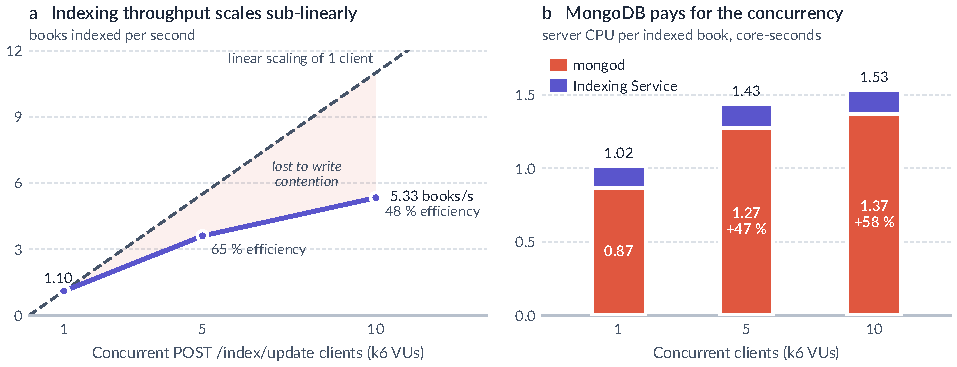
\includegraphics[width=\textwidth]{fig2_indexing_throughput}
  \caption{Indexing benchmark, \route{POST /index/update} on the 20-book corpus
  (official session, one Indexing replica, eight-slot admission bound).
  (a) Measured throughput against linear scaling of the single-client rate
  (dashed); the shaded area is the throughput lost relative to linear scaling,
  and the labels give the parallel efficiency. (b) CPU consumed per indexed
  book, from the \code{docker stats} samples divided by the throughput
  (utilisation law): the \code{mongod} share grows by 58\% from one to ten
  clients while the Indexing Service's own cost stays flat.}
  \label{fig:indexing}
\end{figure}

\begin{table}[htbp]
  \centering
  \footnotesize
  \caption{\route{POST /index/update} under concurrent load: throughput and
  latency per concurrency level (hold phases of 30~s, 20-book corpus, no
  errors). Speed-up and parallel efficiency are relative to one client. With
  33 to 160 updates per level, the 99th percentile rests on few samples.}
  \label{tab:indexing}
  \begin{tabular}{@{}rrrrrrrrrrr@{}}
    \toprule
    VUs & Updates & Books/s & Speed-up & Efficiency & Mean & Median & p90 & p95 & p99 & Max \\
    & & & & & \multicolumn{6}{c}{(ms)} \\
    \midrule
    1  & 33  & 1.10 & 1.00 & 100\% & 919   & 849   & 1{,}520 & 1{,}692 & 2{,}109 & 2{,}298 \\
    5  & 108 & 3.60 & 3.27 & 65\%  & 1{,}370 & 1{,}335 & 2{,}535 & 2{,}904 & 3{,}410 & 3{,}452 \\
    10 & 160 & 5.33 & 4.85 & 48\%  & 1{,}904 & 1{,}889 & 3{,}005 & 3{,}189 & 4{,}078 & 4{,}174 \\
    \bottomrule
  \end{tabular}
\end{table}

\begin{table}[htbp]
  \centering
  \footnotesize
  \caption{Resource use during the indexing benchmark (mean over each hold
  phase; memory as mean and, in parentheses, maximum).}
  \label{tab:indexing-resources}
  \begin{tabular}{@{}rrrrrrrr@{}}
    \toprule
    & \multicolumn{3}{c}{CPU (logical cores)} & \multicolumn{2}{c}{CPU per book (core-s)} & \multicolumn{2}{c}{Memory (MiB)} \\
    \cmidrule(lr){2-4}\cmidrule(lr){5-6}\cmidrule(l){7-8}
    VUs & \code{mongod} & Indexing & Total (host) & \code{mongod} & Indexing & Indexing & \code{mongod} \\
    \midrule
    1  & 0.96 & 0.16 & 1.12 (9\%)  & 0.87 & 0.15 & 22 (26)  & 233 (234) \\
    5  & 4.59 & 0.58 & 5.17 (43\%) & 1.27 & 0.16 & 64 (81)  & 240 (245) \\
    10 & 7.31 & 0.84 & 8.15 (68\%) & 1.37 & 0.16 & 95 (115) & 268 (398) \\
    \bottomrule
  \end{tabular}
\end{table}

\paragraph{Sub-linear scaling.}
Ten concurrent updates index 5.33~books/s, $4.85\times$ the single-client rate
of 1.10~books/s, so parallel efficiency falls from 65\% at five clients to
48\% at ten (\cref{fig:indexing}a). The gap to linear scaling is not lost work:
all 423 timed updates succeeded, and the mean latency of every level agrees
with Little's law, $R = N/X$ (0.91, 1.39 and 1.88~s predicted against 0.92,
1.37 and 1.90~s measured). The extra latency is therefore time spent waiting
or contending. Part of it is designed: at ten clients the handler admits eight
updates and the other two wait for a slot.

\paragraph{Contention, not capacity.}
A capacity limit and a contention limit look alike on a throughput curve, but
the utilisation law separates them. If indexing were capacity-bound, the CPU
cost of a book would stay constant and throughput would stop only when the
host ran out of CPU. Neither happens. At ten clients the stack uses 8.15 of
the 12 logical CPUs (68\%), yet throughput has already flattened; and the cost
of a book is not constant but rises from 1.02 to 1.53 core-seconds
(\cref{fig:indexing}b). All of that growth is inside \code{mongod}, whose cost
per book grows by 47\% at five clients and 58\% at ten, while the Indexing
Service spends a flat 0.15--0.16 core-seconds per book on reading, tokenising
and encoding the writes. Measured against the single-client cost, about one
core-second in three that the stack consumes at ten clients is overhead of
concurrency: at the single-client cost, the same 8.15 cores would have indexed
8.0~books/s instead of 5.33.

The mechanism is the write amplification of the data model
(\cref{sec:decision-storage}): each update rewrites thousands of posting
arrays, and the books of the corpus share most of their common terms, so
concurrent updates write the same term documents. Serialised document writes
and retried write conflicts inside the storage engine are consistent with a
per-book cost that grows with concurrency; the attribution remains a
hypothesis, because \code{serverStatus} counters were not recorded
(\cref{sec:validity}).

\paragraph{The write path in isolation.}
The micro-benchmark \code{IndexBookRealBook} re-indexes book 1342 through the
real write path on an otherwise empty datamart: 636.9~ms per book ($\pm$2\%,
95\% confidence), for 6{,}576 distinct terms and 58{,}860 tokens, with 42.4~MiB
and 444{,}400 allocations per call on the client side. Because every posting
array holds a single entry in this benchmark, its cost is the per-term overhead
of the update pipeline, not the length of the lists. Tokenising a book costs
13.7~ms on one thread (\cref{tab:micro}), about 2\% of the write. Indexing time
is therefore dominated by datamart writes, and tokenising faster would not
help.

\paragraph{Full rebuild.}
In the rebuild-lease experiment, replica A rebuilt the 383-book datalake in
8~min 0.9~s (0.80~books/s through the single-writer rebuild path). Replica B's
overlapping request was answered \code{409 rebuild\_in\_progress} in under a
second, and its retry after the lease was released succeeded in 7~min 54.5~s
(0.81~books/s).

\subsection{Query latency and concurrency}
\label{sec:bench-search}

\Cref{fig:search} plots the search benchmark with one Search replica against the
operational bounds of \cref{sec:setup}; \cref{tab:search} lists both replica
configurations. Neither run produced an error: 33{,}131 and 32{,}819
successful queries, all of which passed the k6 checks on status, schema, page
size and echoed pagination. About 30.5\% of the responses were empty pages
(no-match words, stop words, restrictive filters or offsets past the end), an
intended part of the mix.

\begin{figure}[tbp]
  \centering
  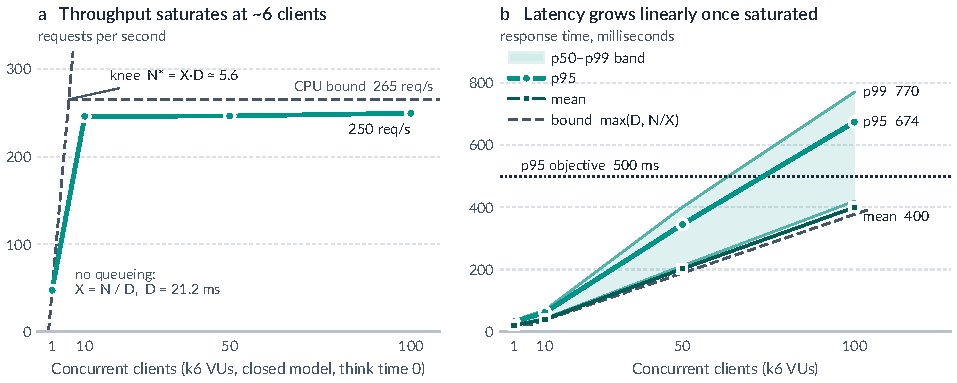
\includegraphics[width=\textwidth]{fig1_query_latency}
  \caption{\route{GET /search} through nginx, one Search replica, 300-book
  datamart, 30~s hold per level. (a) Throughput against the asymptotic bounds:
  without queueing, $X = N/D$ with $D = 21.2$~ms, the response time of a lone
  query; the CPU bound $X_{\max} = 12 / D_{\text{cpu}} = 265$~req/s follows from the
  45.2 core-ms of server CPU that one query costs at saturation
  (\cref{fig:cpu}c). The bounds meet at the knee $N^{*} \approx 5.6$ clients.
  (b) Latency distribution: the band spans the median to the 99th percentile;
  the mean stays 6--7\% above the lower bound $\max(D, N/X_{\max})$, and the 95th
  percentile crosses the 500~ms objective between 50 and 100 clients.}
  \label{fig:search}
\end{figure}

\begin{table}[htbp]
  \centering
  \footnotesize
  \caption{\route{GET /search} through nginx with one and two Search replicas:
  steady-state throughput and latency per concurrency level (hold phases of
  30~s, 300-book datamart, 0\% errors). $N/X$ is the mean latency Little's law
  predicts from the measured throughput.}
  \label{tab:search}
  \begin{tabular}{@{}rcrrrrrrrrr@{}}
    \toprule
    VUs & Replicas & Requests & Req/s & Mean & $N/X$ & Median & p90 & p95 & p99 & Max \\
    & & & & \multicolumn{7}{c}{(ms)} \\
    \midrule
    1   & 1 & 1{,}417 & 47.23  & 20.8  & 21.2  & 22.1  & 29.4  & 31.8  & 35.8  & 51.3 \\
        & 2 & 1{,}473 & 49.10  & 20.0  & 20.4  & 21.4  & 28.6  & 30.4  & 33.0  & 44.1 \\
    \addlinespace
    10  & 1 & 7{,}382 & 246.07 & 40.1  & 40.6  & 42.6  & 57.8  & 61.8  & 69.2  & 95.6 \\
        & 2 & 7{,}365 & 245.50 & 40.2  & 40.7  & 42.6  & 58.3  & 62.5  & 70.3  & 100.4 \\
    \addlinespace
    50  & 1 & 7{,}393 & 246.43 & 202.3 & 202.9 & 211.9 & 315.9 & 345.0 & 400.6 & 506.3 \\
        & 2 & 7{,}262 & 242.07 & 206.0 & 206.6 & 214.5 & 323.7 & 355.6 & 416.8 & 700.9 \\
    \addlinespace
    100 & 1 & 7{,}490 & 249.67 & 399.7 & 400.5 & 419.3 & 624.4 & 673.7 & 769.7 & 931.0 \\
        & 2 & 7{,}431 & 247.70 & 403.0 & 403.7 & 424.5 & 625.3 & 680.4 & 767.6 & 971.6 \\
    \bottomrule
  \end{tabular}
\end{table}

\paragraph{Saturation happens at about six clients.}
One client obtains 47.2~req/s; ten obtain 246~req/s, only $5.2\times$ more;
50 and 100 clients obtain no more at all (246--250~req/s). The bounds of
\cref{fig:search}a locate the transition without fitting anything. A lone query
takes $D = 21.2$~ms, so with no queueing $N$ clients could push $N/D =
47.2\,N$~req/s. One query consumes 45.2 core-milliseconds of server CPU at
saturation, so the 12 logical CPUs cap throughput at $X_{\max} = 265$~req/s. The
two bounds meet at $N^{*} = X_{\max} D \approx 5.6$ clients: below that
concurrency a client rarely waits, above it every additional client only
lengthens the queue. The measured plateau reaches 93--94\% of $X_{\max}$, and the
remaining CPU went to the load generator, the Docker daemon and WSL2, which
were not sampled. The knee lies close to the six physical cores of the host,
for the reason explained in \cref{sec:bench-resources}.

\paragraph{Latency past the knee is pure queueing.}
Above $N^{*}$, the mean grows linearly with the number of clients, from 40~ms at
10 clients to 202~ms at 50 and 400~ms at 100 (\cref{fig:search}b). Two checks
show that the system behaves as one clean bottleneck. First, the means agree with
Little's law to within 2\% at every level (\cref{tab:search}), so no work is
lost or hidden. Second, they stay 6--7\% above the asymptotic lower bound
$N/X_{\max}$, and that gap is constant: throughput does not fall as the queue
grows, so there is no thrashing, lock convoy or retry storm, only waiting. The
tail widens with the queue: the 95th percentile is 1.44 to 1.63 times the
median and the 99th 1.62 to 1.89 times, because a query that lands behind a
long aggregation waits for it.

\paragraph{Service objectives.}
The script's objectives are a mean below 200~ms over the whole run and a 95th
percentile below 500~ms at every level. The first holds (194.0 and 195.8~ms
over the two runs). The second holds up to 50 clients (345 and 356~ms) and
fails at 100 (674 and 680~ms), which is why k6 exits with code 99; every
availability threshold (fewer than 1\% failed requests, more than 99\% passed
checks) passed. With zero think time the benchmark is deliberately harsher
than real traffic. Little's law with a think time $Z$ between a user's
searches gives the population a saturated service supports:
$N \approx X\,(R + Z) \approx 1{,}250$ users who search every 5~s. This is an
estimate derived from the law, not a measurement.

\subsection{CPU and memory utilisation per process and host}
\label{sec:bench-resources}

\Cref{fig:cpu} follows CPU and memory of every container through the
one-replica search run, and divides the CPU by the throughput to obtain the
cost of one query in each process. \Cref{tab:resources} gives the per-level
means for both replica configurations.

\begin{figure}[tbp]
  \centering
  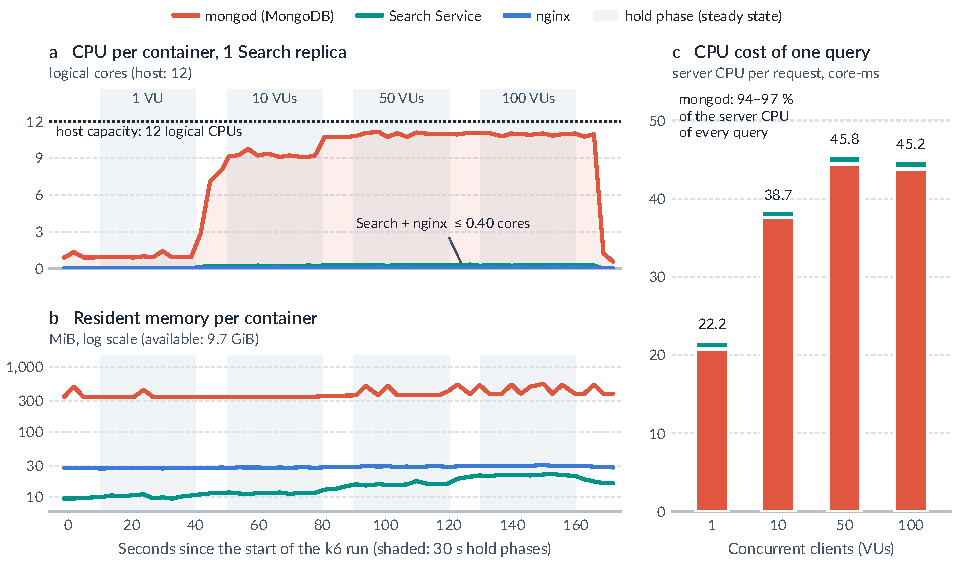
\includegraphics[width=\textwidth]{fig3_resource_utilisation}
  \caption{Resources during the one-replica search benchmark (\code{docker stats},
  one sample about every 3~s; shaded: the 30~s hold phases whose means enter
  \cref{tab:resources}). (a) CPU per container: \code{mongod} rises from one core
  to 10.9 of the 12 logical CPUs (dotted) while the Search Service and nginx
  together never exceed 0.40 cores. (b) Resident memory on a logarithmic scale:
  every process stays two orders of magnitude below the 9.7~GiB available.
  (c) Server CPU per query, CPU of each container divided by the throughput of
  the level (utilisation law): \code{mongod} accounts for 94--97\% of it, and
  the cost doubles from one client to saturation. The two-replica run is
  indistinguishable (\cref{tab:resources}).}
  \label{fig:cpu}
\end{figure}

\begin{table}[htbp]
  \centering
  \footnotesize
  \caption{CPU (logical cores) and resident memory (MiB, mean and maximum) per
  container during the hold phases of the search benchmark. The host provides
  12 logical cores; with two replicas, the Search columns give replica 1 +
  replica 2. Values are those written by the chart script to
  \code{chart\_data.csv}.}
  \label{tab:resources}
  \begin{tabular}{@{}crrrrrrrr@{}}
    \toprule
    & & \multicolumn{4}{c}{CPU (logical cores)} & \multicolumn{3}{c}{Memory (MiB)} \\
    \cmidrule(lr){3-6}\cmidrule(l){7-9}
    Replicas & VUs & \code{mongod} & Search & nginx & Total (host) & \code{mongod} & Search & nginx \\
    \midrule
    1 & 1   & 0.98  & 0.05 & 0.02 & 1.05 (9\%)   & 356 (442) & 10      & 28 \\
      & 10  & 9.25  & 0.22 & 0.06 & 9.53 (79\%)  & 348 (348) & 11      & 28 \\
      & 50  & 10.95 & 0.27 & 0.07 & 11.29 (94\%) & 403 (511) & 16      & 29 \\
      & 100 & 10.94 & 0.27 & 0.08 & 11.29 (94\%) & 448 (547) & 22      & 30 \\
    \addlinespace
    2 & 1   & 0.99  & 0.03 + 0.03 & 0.02 & 1.06 (9\%)   & 387 (388) & 14 + 9  & 28 \\
      & 10  & 9.23  & 0.13 + 0.13 & 0.06 & 9.55 (80\%)  & 390 (391) & 14 + 11 & 28 \\
      & 50  & 10.85 & 0.14 + 0.15 & 0.08 & 11.23 (94\%) & 441 (545) & 16 + 13 & 29 \\
      & 100 & 10.93 & 0.14 + 0.14 & 0.07 & 11.28 (94\%) & 474 (579) & 18 + 17 & 30 \\
    \bottomrule
  \end{tabular}
\end{table}

\paragraph{The datamart consumes the host.}
With one client, \code{mongod} already uses one full core, and its 20.8~ms of
CPU per query coincide with the 20.8~ms mean response: one aggregation runs on
one core for practically the whole request. From 10 clients onwards
\code{mongod} uses 9.2 to 11.0 cores, and from 50 clients all containers
together use 94\% of the host (\cref{fig:cpu}a); the remainder is shared by the
load generator, the Docker daemon and WSL2, so the host is effectively
CPU-saturated. The Search process uses 0.05 to 0.27 cores, about 1~ms of CPU
per query, and nginx 0.2 to 0.4~ms. \code{mongod} accounts for 93.5\% of the
server-side CPU of a query with one client and 97\% from ten clients onwards
(\cref{fig:cpu}c). The Search Service is a thin translation layer; the search
engine, in terms of where the cycles go, is the aggregation inside MongoDB.

\paragraph{Why the cost of a query doubles under load.}
The CPU cost of one query is not constant: it rises from 20.8 core-ms with one
client to 37.6 with ten and 44.4 with fifty (\cref{fig:cpu}c), a factor of 2.1.
Between 10 and 50 clients \code{mongod} received 1.7 more cores but served no
more queries. The factor of about two is the signature of simultaneous
multithreading: the host has six physical cores presented as 12 logical CPUs,
and once more aggregations are runnable than there are physical cores, two
hardware threads share the execution units of one core, each progressing at
roughly half speed while \code{docker stats} charges both as busy. The
consistent arithmetic is that six physical cores running one aggregation each at
the single-client cost would deliver $6 / 20.8~\text{ms} \approx 290$~req/s; the
measured plateau is 86\% of that, a gap compatible with a lower all-core clock
than the single-core turbo and with the CPU taken by k6. Clock frequency and
hardware counters were not recorded, so this mechanism is a well-supported
hypothesis rather than a measurement. Its practical reading matters more than
its proof: on this host, \emph{logical} CPUs are not capacity, and the
effective processor count for aggregation-heavy work is closer to six than to
twelve.

\paragraph{Why one query costs so much.}
The datamart micro-benchmarks (\cref{tab:datamart-micro}) isolate the
aggregation on a synthetic 300-book datamart. Fetching the posting list of a
term contained in every book takes 0.60~ms, but the full search aggregation for
that term takes 26.2~ms, $43\times$ more. The cost lies in the stages after the
intersection: one \code{\$lookup} sub-pipeline per candidate book, followed by
a \code{\$facet} that counts and sorts every match. A common term has a
candidate for almost every book, so the join runs about 300 times per query.
Adding the three metadata filters makes the query \emph{slower} (37.9~ms,
$+45\%$), because the filters are evaluated per candidate inside the lookup,
after the point read by \code{\_id}, instead of pruning candidates through the
filter indexes. This reading of the query plan is an inference from the
pipeline's structure; \code{explain()} output was not recorded.

\begin{table}[htbp]
  \centering
  \footnotesize
  \caption{Datamart micro-benchmarks against the live server
  (\code{go test -bench}, 10 samples, median $\pm$ 95\% confidence interval from
  \code{benchstat}; \code{GOMAXPROCS} = 12). The read benchmarks use a synthetic
  300-book datamart in which the queried term occurs in every book; bytes and
  allocations are those of the Go client.}
  \label{tab:datamart-micro}
  \begin{tabularx}{\textwidth}{@{}l>{\raggedright\arraybackslash}Xrrr@{}}
    \toprule
    Benchmark & Operation & Time per op & Bytes/op & Allocs/op \\
    \midrule
    \code{PostingsForTerms} & Posting list of one term & 603.0~$\mu$s $\pm$ 5\% & 54.4~KiB & 1{,}973 \\
    \code{SearchBooksWithoutFilters} & Full search aggregation, no filter & 26.18~ms $\pm$ 3\% & 34.1~KiB & 773 \\
    \code{SearchBooksWithAllFilters} & Same, with author, language and year & 37.90~ms $\pm$ 12\% & 35.6~KiB & 679 \\
    \code{IndexBook} & Re-index a synthetic 7-token book & 4.544~ms $\pm$ 4\% & 42.4~KiB & 582 \\
    \code{IndexBookRealBook} & Re-index book 1342 (6{,}576 terms) & 636.9~ms $\pm$ 2\% & 42.4~MiB & 444{,}400 \\
    \bottomrule
  \end{tabularx}
\end{table}

\paragraph{Memory is not the constraint, yet.}
\Cref{fig:cpu}b uses a logarithmic axis because the three processes differ by
two orders of magnitude. \code{mongod} held 348--474~MiB on average with
transient peaks up to 547~MiB (579~MiB with two replicas) during the saturated
holds, consistent with per-query sort and \code{\$facet} buffers being
allocated and released; the Search process grew from 10 to 22~MiB with
concurrency, as each in-flight request holds a goroutine stack and a response
buffer; nginx stayed at 28--31~MiB; the Indexing Service stayed below 120~MiB
(\cref{tab:indexing-resources}). The whole stack used less than 0.7~GiB of the
9.7~GiB available. The thread counts reflect the two concurrency models of
\cref{sec:replicas-threads}: \code{mongod} grew from about 45 to 155 threads (209
in the two-replica run) as connections were opened, one thread per connection,
while each Search process stayed at 13 to 24 operating-system threads for up to
100 concurrent requests. A 300-book datamart fits entirely in MongoDB's cache;
memory becomes relevant when the working set of posting arrays outgrows it,
which this corpus does not exercise.

\subsection{Effects of replication}
\label{sec:bench-replication}

The replica experiment (item RF~8 of the group's Stage~2 audit checklist, the
label used in \code{docker-compose.replicas.yml} and \code{deploy/nginx/nginx.conf})
repeated the identical k6 profile, with the same seed, datamart, host and
proxy, once with one and once with two Search replicas behind nginx; the
replica count was the only variable (\cref{fig:replication}).

\begin{figure}[tbp]
  \centering
  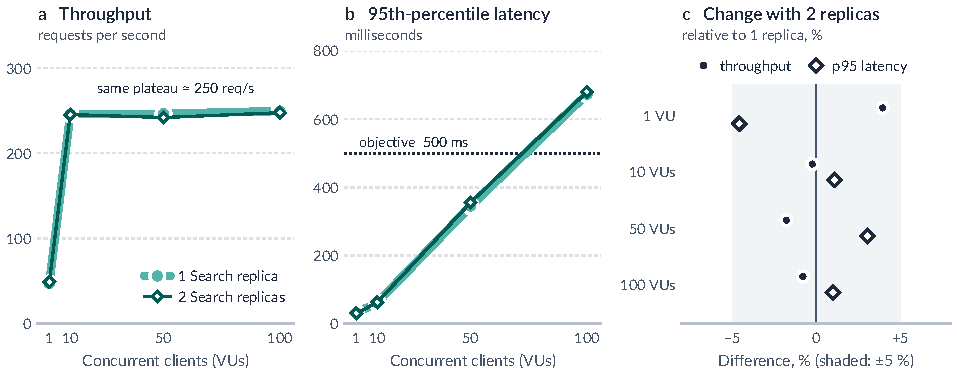
\includegraphics[width=\textwidth]{fig4_replication}
  \caption{One versus two Search replicas behind nginx (\code{least\_conn}),
  identical k6 profile, seed, datamart and host. (a)~Throughput and (b)~95th
  percentile latency: the thin dark line of the two-replica run lies inside the
  thick light line of the one-replica run at every level. (c)~Relative change
  with two replicas; the shaded $\pm 5\%$ band is a visual reference, not a
  measured confidence interval. No change has a consistent sign.}
  \label{fig:replication}
\end{figure}

\paragraph{The load was distributed.}
nginx split the work evenly: from 10 clients upwards the two replicas used the
same CPU within 7\% (0.132/0.127, 0.144/0.153 and 0.137/0.138 cores at 10, 50
and 100 clients), and the \code{X-Upstream} header alternated between the two
container addresses. Their combined CPU (0.26--0.30 cores) is what one replica
used alone (0.22--0.27 cores): the work was divided between two processes, not
reduced.

\paragraph{Throughput and latency did not change.}
Throughput changed by $+4.0\%$, $-0.2\%$, $-1.8\%$ and $-0.8\%$ at 1, 10, 50 and 100
clients, and the 95th percentile by $-4.6\%$, $+1.1\%$, $+3.1\%$ and $+1.0\%$
(\cref{fig:replication}c). Every difference lies within $\pm 5\%$, the sign flips
between levels, and the one-client run, where two replicas look best, is the
level at which no replica is busy. With one run per configuration these
differences are indistinguishable from run-to-run variation, so no effect of
replication is detectable; \code{mongod}'s CPU changed by less than 1\% at
every level.

\paragraph{Why it could not change.}
The asymptotic bound explains the null result quantitatively. $X_{\max} = m /
D_{\text{cpu}}$ depends on the processors of the host and on the CPU one query
consumes; a second Search replica changes neither, because it only splits the
Search share of $D_{\text{cpu}}$, 1.1 of 45.2 core-ms, between two processes.
Even if the Search and nginx tiers cost nothing at all, the bound would rise
from 265 to 274~req/s, $+3\%$: that is the most any amount of Search
replication can buy on this host. Replication did change one property of the
datamart: each replica brings its own connection pool, so \code{mongod} ran up to
209 threads instead of 155, with no more CPU to run them. The measurement
thus confirms the expectation of \cref{sec:decision-scaling}.

\subsection{Effects of threading}
\label{sec:bench-threads}

\Cref{fig:threads} contrasts three kinds of work under added threads or workers:
CPU-bound text processing, network-bound ingestion and datamart-bound
operations.

\begin{figure}[tbp]
  \centering
  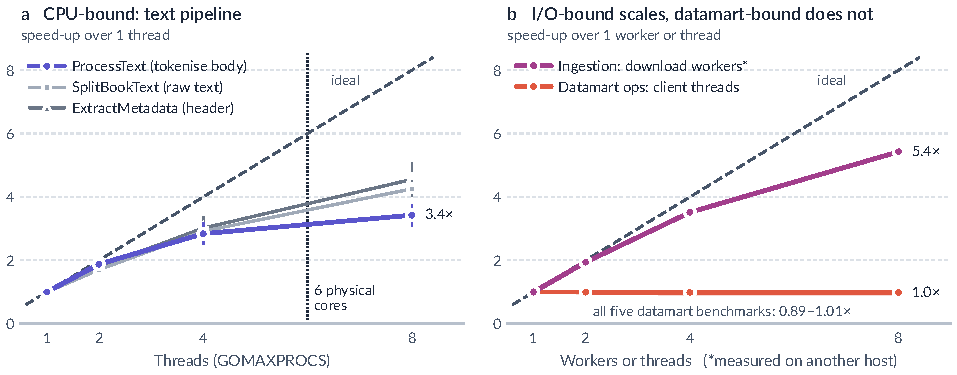
\includegraphics[width=\textwidth]{fig5_threading}
  \caption{Threading. (a) The three CPU-bound functions of the indexing
  pipeline run in parallel (\code{b.RunParallel}) over the 383 real books;
  error bars are the 95\% confidence intervals of \code{benchstat} combined for
  the ratio. They scale to $3.4$--$4.6\times$ with eight threads, flattening
  beyond the six physical cores. (b) Network-bound ingestion of 99 real books
  into a cold datalake scales to $5.4\times$ with eight download workers
  (measured on another machine, \cref{tab:workloads}), whereas the five datamart
  micro-benchmarks stay at $0.89$--$1.01\times$ whatever the client's thread
  count: their time is spent inside \code{mongod}. Dashed: ideal linear
  speed-up.}
  \label{fig:threads}
\end{figure}

\begin{table}[htbp]
  \centering
  \footnotesize
  \caption{Text pipeline micro-benchmarks over the 383 real books of the
  datalake, run in parallel by \code{GOMAXPROCS} goroutines
  (\code{b.RunParallel}): median time per operation (10 samples) and speed-up.}
  \label{tab:micro}
  \begin{tabular}{@{}llrrrrrr@{}}
    \toprule
    Function & Input & 1 thread & 2 & 4 & 8 & Speed-up at 8 & Efficiency \\
    \midrule
    \code{ProcessText} & book body & 13.66~ms & 7.27~ms & 4.81~ms & 3.99~ms & $3.42\times$ & 43\% \\
    \code{ExtractMetadata} & header & 23.5~$\mu$s & 13.1~$\mu$s & 7.79~$\mu$s & 5.16~$\mu$s & $4.55\times$ & 57\% \\
    \code{SplitBookText} & raw text & 211~$\mu$s & 124~$\mu$s & 72.5~$\mu$s & 49.7~$\mu$s & $4.25\times$ & 53\% \\
    \bottomrule
  \end{tabular}
\end{table}

\paragraph{CPU-bound work scales, up to the physical cores.}
The three text functions run in parallel without shared state and reach
$3.4\times$ to $4.6\times$ with eight threads (\cref{tab:micro},
\cref{fig:threads}a). Scaling is close to linear up to two threads and flattens
beyond four, as expected on six physical cores with simultaneous
multithreading, the same effect that doubles the cost of a query in
\cref{sec:bench-resources}. \code{ProcessText}, the tokeniser, scales least: it
allocates about 15~MB per book, so memory bandwidth and garbage collection are
plausible further limits. Text processing is in any case not what limits
indexing (\cref{sec:bench-indexing}).

\paragraph{Datamart-bound work does not scale with client threads.}
The datamart micro-benchmarks were swept with \code{-cpu 1,2,4,8}; their
speed-ups stay between 0.89 and 1.01 (\cref{fig:threads}b), and, for example,
\code{SearchBooksWithoutFilters} takes 26.22--26.32~ms at every setting. These
benchmarks issue one request at a time, so the sweep varies the client's thread
count, not the load on the server. The flat result shows that the cost of a
datamart operation is spent in \code{mongod}, not in the Go client; how the
server scales with concurrent requests is what the k6 runs measure.

\paragraph{Network-bound work scales almost linearly.}
Ingestion scales almost linearly up to four download workers ($3.51\times$) and
reaches $5.42\times$ (21.3~books/s) at eight, with the Ingestion process using
on average less than 2\% of the machine's CPU (\cref{tab:ingestion}). Its limit
is the latency of the upstream Gutenberg server, not local resources. Because
the experiment ran on another machine, the shape of the curve is the finding,
not its absolute rates.

\begin{table}[htbp]
  \centering
  \footnotesize
  \caption{Cold-datalake ingestion of 100 real Gutenberg IDs (99 available, one
  answered \code{404 book\_unavailable}); only \code{2xx} answers are counted.
  Host: Intel Core Ultra 7 155H (16 cores), 32~GB, Windows 11.}
  \label{tab:ingestion}
  \begin{tabular}{@{}rrrrrr@{}}
    \toprule
    Workers & Elapsed (s) & Books/s & Speed-up & CPU (machine) & Peak working set \\
    \midrule
    1 & 25.19 & 3.93  & 1.00 & 0.5\% & 83~MB \\
    2 & 12.98 & 7.63  & 1.94 & 0.6\% & 37~MB \\
    4 & 7.17  & 13.81 & 3.51 & 1.1\% & 37~MB \\
    8 & 4.64  & 21.32 & 5.42 & 1.8\% & 47~MB \\
    \bottomrule
  \end{tabular}
\end{table}

\paragraph{Configurations not tested.}
Some combinations remain unmeasured, and the conclusions do not extend to
them. Ingestion and Indexing replicas were not run under load (Indexing ran as
two replicas only in the lease experiment). Every search run went through
nginx, so the proxy's own latency was not isolated. The services'
\code{GOMAXPROCS}, the driver's pool size and the eight-slot bounds were not
varied, and no container ran with CPU or memory limits or pinned to cores.

\subsection{Coordination overhead}
\label{sec:bench-coordination}

The Control Module logs the wall-clock duration of every ingestion and
indexing step it waits for. The time of a run that is \emph{not} spent waiting
on a service step, its worker time minus the step totals, is therefore an upper
bound on the orchestrator's own overhead: claiming, recording progress under
\code{flock}, logging and retry backoff. \Cref{tab:coordination-runs} reports
four runs of 100 books with 1, 2, 4 and 8 workers. These runs predate the
official session and used different ID ranges, so they are reported as a table
of indicative values rather than plotted next to the official curves.

\begin{table}[htbp]
  \centering
  \footnotesize
  \caption{End-to-end orchestration runs (29~October~2026). Step
  means are over the books that entered the pipeline; ``unattributed'' is the
  share of worker time not spent waiting on a service step.}
  \label{tab:coordination-runs}
  \begin{tabular}{@{}rlrrrrrr@{}}
    \toprule
    Workers & IDs & Indexed / failed & Elapsed (s) & Books/s & Ingest step & Index step & Unattributed \\
    \midrule
    1 & 1--100   & 96 / 4   & 219.2 & 0.44 & 0.59~s & 1.41~s & 8.8\% \\
    2 & 101--200 & 78 / 22  & 187.2 & 0.42 & 0.45~s & 2.37~s & 24.9\% \\
    4 & 201--300 & 98 / 2   & 105.8 & 0.93 & 0.44~s & 3.64~s & 3.6\% \\
    8 & 301--400 & 100 / 0  & 90.9  & 1.10 & 0.43~s & 6.65~s & 2.6\% \\
    \bottomrule
  \end{tabular}
\end{table}

The orchestrator itself is cheap: in the run without failures, at most 2.6\% of
worker time was spent outside service calls, and that bound also includes the
idle tail at the end of the run. The higher shares at one and two workers come
from retry backoff: those runs predate the realignment of the ingestion entry
point with its specification, when books that Gutenberg does not serve were
answered with \code{503} and retried as transient before being recorded as
failed (22 such books in the two-worker run). The real coordination cost is the
waiting. Going from one to eight workers raised end-to-end throughput only
$2.5\times$ (0.44 to 1.10~books/s), because the mean index step grew
$4.7\times$ (1.41 to 6.65~s), the same datamart contention that
\cref{fig:indexing}b measures as a rising per-book cost, while the mean
ingestion step stayed between 0.43 and 0.59~s. In other words, adding workers
to the coordinator moves the queue from the coordinator into MongoDB; it does
not shorten it.

\subsection{Bottlenecks and performance limits of the single host}
\label{sec:bench-limits}

The figures rank the limits of the deployment in the order in which they bind:

\begin{enumerate}
  \item \textbf{Search: datamart CPU.} About 250~req/s from ten clients on,
  with the knee at $N^{*} \approx 5.6$ clients (\cref{fig:search,fig:cpu}).
  \item \textbf{Host CPU, counted in physical cores.} Six physical cores, not
  twelve logical CPUs, are the real capacity (\cref{sec:bench-resources}).
  \item \textbf{Indexing: write contention in the datamart, not capacity.} 48\%
  efficiency at ten updates with the host 68\% busy (\cref{fig:indexing}).
  \item \textbf{Ingestion: the upstream network.} Downloads parallelise well at
  negligible local cost (\cref{fig:threads}b).
  \item \textbf{Memory: not yet a limit.} Under 0.7 of the 9.7~GiB available
  for a 300-book datamart (\cref{fig:cpu}b).
  \item \textbf{Coordination: not a throughput limit.} At most 2.6\% of worker
  time (\cref{tab:coordination-runs}).
  \item \textbf{Co-location.} One CPU shared by load generator, datamart and
  services, so the ceiling belongs to the whole host.
\end{enumerate}

\subsection{Threats to validity}
\label{sec:validity}

\begin{itemize}
  \item \textbf{One run per configuration.} The k6 results have no
  run-to-run confidence intervals; differences of a few percent, such as those
  between one and two replicas, cannot be distinguished from noise.
  \item \textbf{Short holds.} The 30~s hold phases capture steady state but
  not long-run effects such as cache eviction or the growth of the WiredTiger
  cache.
  \item \textbf{Co-located load generator.} k6 competed with the services for
  CPU, especially at 100 VUs, and its own consumption was not sampled.
  \item \textbf{Sampling.} \code{docker stats} yields one sample about every
  3~s, each covering a short interval, so the per-level CPU values are means
  of 8 to 10 samples. During the saturated holds the coefficient of variation
  of \code{mongod}'s CPU stayed below 2.5\%; the small Search and nginx
  readings vary more (up to about 30\%), which is why their per-query costs are
  quoted to one significant digit.
  \item \textbf{Virtualisation and power management.} WSL2 adds a hypervisor
  layer, and CPU frequency was neither fixed nor recorded; the simultaneous
  multithreading explanation of \cref{sec:bench-resources} rests on that
  missing measurement.
  \item \textbf{Warm caches.} The page cache and MongoDB's cache were warm,
  and the indexing benchmark re-indexed books already present.
  \item \textbf{Corpus.} The search datamart was seeded by walking Gutenberg
  IDs upwards from 1 until 300 books were published; results may shift on a
  corpus with a different term distribution or size.
  \item \textbf{Unrecorded internals.} MongoDB's \code{serverStatus} counters
  and \code{explain()} plans were not captured; attributions to write conflicts
  and to the lookup stage are inferences.
  \item \textbf{Heterogeneous evidence.} The ingestion experiment ran on
  another machine, the coordination runs before the official session, and the
  API validation against MongoDB~8.3.7; these results are never compared
  numerically with the official ones.
\end{itemize}

\section{Conclusions and Future Improvements}
\label{sec:conclusions}

Stage~2 met its objectives: the Stage~1 data layer now runs as cooperating
services with documented and validated contracts, an explicit coordination
mechanism and a measured performance envelope. The measurements also close the
question Stage~1 left open: MongoDB serves several independent processes
correctly under concurrent access, and on a single host it is the first
component to saturate on both the read and the write path
(\cref{sec:bench-limits}), the fact from which the design of Stage~3 follows.

\subsection{Strengths}
\label{sec:strengths}

\begin{itemize}
  \item \textbf{Contracts that are specified and verified.} The OpenAPI
  documents are generated from the code, and the running stack passes every API
  check, automated test and end-to-end script (\cref{sec:validation,sec:testing}).
  \item \textbf{Coordination that tolerates failures.} Ingestion before
  indexing is enforced twice, half-indexed books are invisible, rebuilds are
  serialised across replicas, and idempotency turns a crash between a call and
  its record into a harmless replay (\cref{sec:coordination,sec:readiness}).
  \item \textbf{Graceful saturation.} Past the knee, throughput holds its
  plateau and latency grows exactly as queueing predicts, with no failed
  request even at 100 clients (\cref{sec:bench-search}).
  \item \textbf{A lean service tier.} The Go services and nginx account for only
  a few percent of the CPU of a query; the cost lies in the datamart
  (\cref{sec:bench-resources}).
  \item \textbf{Concurrency that is bounded and measured.} Semaphores,
  timeouts and context propagation keep overload from exhausting resources,
  and CPU- and network-bound work scale with threads as expected
  (\cref{sec:bench-threads}).
  \item \textbf{Reproducible evidence.} Every figure is regenerated by one
  script from committed raw files (\cref{sec:provenance}).
\end{itemize}

\subsection{Weaknesses}
\label{sec:weaknesses}

\begin{itemize}
  \item \textbf{One datamart server bounds both paths.} Search saturates early
  and misses its 95th-percentile objective at 100 clients, indexing scales
  sub-linearly, and Search replicas cannot help on one host
  (\cref{sec:bench-limits}).
  \item \textbf{An expensive query plan.} The per-candidate \code{\$lookup} and
  the \code{\$facet} dominate the cost of a search, and metadata filters make it
  slower rather than faster (\cref{sec:bench-resources}).
  \item \textbf{Write amplification and contention.} The one-document-per-term
  layout rewrites thousands of posting arrays per book, concurrent updates
  collide on shared term documents, and common terms approach the document
  size ceiling (\cref{sec:decision-storage,sec:bench-indexing}).
  \item \textbf{Per-process coordination state.} The rebuild replay list, the
  ingestion single-flight map and the Control Module's claim cursor live in
  memory, so they hold for one process only (\cref{tab:local-assumptions}).
  \item \textbf{One coordinator.} New books stop entering the pipeline while
  the Control Module is down (\cref{sec:decision-coordination}).
  \item \textbf{Limited evidence.} Single runs, a co-located load generator and
  unrecorded server counters limit the precision of the results
  (\cref{sec:validity}).
\end{itemize}

\subsection{From the measurements to the Stage 3 evolution}
\label{sec:evidence-to-design}
\label{sec:stage3}

The figures cannot show how the system will scale on a cluster
(\cref{sec:introduction}), but they rule options out and set priorities.
\Cref{tab:evidence-stage3} orders the Stage~3 work by expected impact and pairs
each decision with the measured fact behind it and with the acceptance check
that will confirm it, using the same benchmark and the same figure, so that
Stage~3 is evaluated against Stage~2 like for like.

\begin{table}[htbp]
  \centering
  \footnotesize
  \caption{Prioritised improvements for Stage~3: the measured facts behind each
  decision, and how each decision will be verified with the same benchmarks and
  figures.}
  \label{tab:evidence-stage3}
  \begin{tabularx}{\textwidth}{@{}r>{\raggedright\arraybackslash}p{3.4cm}>{\raggedright\arraybackslash}p{2.9cm}>{\raggedright\arraybackslash}X>{\raggedright\arraybackslash}p{3.1cm}@{}}
    \toprule
    \# & Measured fact & What it implies & Stage 3 decision & Acceptance check \\
    \midrule
    1 & \code{mongod}: 94--97\% of the CPU of a query; ceiling 250~req/s at
      $N^{*} \approx 6$ clients; full aggregation $43\times$ the cost of
      fetching postings (\cref{fig:search,fig:cpu,tab:datamart-micro}) &
      The read ceiling is a property of the datamart, and a cheaper query raises
      it on every node &
      Rank the intersected postings and join only the requested page; filter on
      denormalised or index-backed attributes; cache hot queries in the Search
      replicas, keyed by index version; then scale reads with replica-set
      secondaries or shards &
      \cref{fig:cpu}c: lower core-ms per query, checked with \code{explain()};
      \cref{fig:search}a: plateau scales with data nodes \\
    \addlinespace
    2 & Indexing: 48\% efficiency with the host 68\% busy; per-book
      \code{mongod} cost $+58\%$ (\cref{fig:indexing}) &
      Contention on shared term documents, not lack of CPU: more cores on one
      server would not help &
      (term, book) posting documents (\code{docs/mongodb.md}), which also remove
      the 16~MB ceiling; shard
      key hashed on the term; batched, unordered writes; indexing tasks
      partitioned by book &
      \cref{fig:indexing}b: per-book cost flat ($\le 10\%$ growth) from 1 to 10
      clients; efficiency $\ge 80\%$ at 10 \\
    \addlinespace
    3 & Query cost doubles past six clients on 6 physical / 12 logical cores;
      single runs; server counters and CPU frequency not recorded
      (\cref{fig:cpu}c, \cref{sec:validity}) &
      Logical CPUs overstate capacity, and two attributions remain hypotheses &
      Size data nodes by physical cores; pin or limit containers; run k6 on its
      own node; record \code{serverStatus}, query plans and CPU frequency;
      repeat every configuration at least three times &
      Cost per query constant across load levels; every figure with confidence
      intervals \\
    \addlinespace
    4 & Orchestrator overhead $\le 2.6\%$; index step $4.7\times$ longer with 8
      workers (\cref{tab:coordination-runs}) &
      Central coordination is an availability problem, not a throughput one &
      A tasks collection with leases replacing the control files and the
      in-memory claim, or a broker with consumer groups &
      Throughput unchanged when one coordinator is killed mid-run \\
    \addlinespace
    5 & Deep offsets cost datamart work proportional to the offset
      (\cref{sec:decision-api}) &
      Offset pagination degrades as the corpus grows &
      Keyset pagination, continuing after the last returned score and book ID &
      Page latency independent of the offset \\
    \addlinespace
    6 & Two Search replicas: $|\Delta| \le 5\%$; at most $+3\%$ possible on one
      host (\cref{fig:replication}) &
      Stateless replicas add availability, not throughput, while the datamart is
      shared &
      Keep $\ge 2$ Search replicas on different nodes for availability; add more
      only when \cref{fig:cpu}c shows the Search tier is the bottleneck &
      Repeat \cref{fig:replication} on the cluster: throughput should rise with
      replicas once data nodes scale \\
    \addlinespace
    7 & Ingestion $5.4\times$ with 8 workers at $<2\%$ CPU (\cref{fig:threads}b) &
      Network-bound; scales with concurrency, not with machines &
      Keep one Ingestion replica per node with a worker pool; rate-limit towards
      Gutenberg &
      Books/s versus workers per node \\
    \bottomrule
  \end{tabularx}
\end{table}

\paragraph{Why a cheaper query comes first.}
Because the read bound is $X_{\max} = m / D_{\text{cpu}}$, read capacity can grow
through more processors $m$ (data nodes that serve reads) or a smaller demand
$D_{\text{cpu}}$ per query, and the second multiplies the first: every halving of
the 21~ms per query doubles the ceiling of every data node. As a rough
illustration, sustaining 1{,}000~req/s on today's plan would need at least four
six-core data nodes serving reads, an extrapolation of the bound rather than a
measurement. Once the datamart scales, the Search tier, at about 1~ms of CPU per
query or roughly 1{,}000 queries per second per core, becomes the next limit,
and only then do Search replicas on separate nodes raise throughput.

\paragraph{Cross-machine communication and storage access.}
The HTTP/JSON contracts carry over unchanged, because every address already
comes from configuration, and each local mechanism is replaced as listed in
\cref{tab:local-assumptions}: for example Kubernetes services or Consul for
discovery, and MinIO or S3 for the datalake, with a completion marker object
written last. Timeouts and retry budgets must be recalibrated from the measured
percentiles rather than single-host defaults; the 21~ms service time of a lone
query leaves room for a few milliseconds of network per hop. Idempotency keeps
retries over an unreliable network safe, and jitter in the backoff prevents
synchronised retry storms. MongoDB becomes a replica set of at least three
nodes for availability and read scaling, with the inverted index laid out and
sharded as in row~2 of \cref{tab:evidence-stage3}.

\paragraph{Distribution of tasks and requests.}
Pipeline work becomes claimable tasks, either documents claimed atomically
under a lease or \code{BookDownloaded} and \code{BookIndexed} events
partitioned by book ID, so that the updates of one book stay ordered and
several Control instances (or none, under choreography) can share the work
without duplicating it. Search requests are balanced over replicas on several
nodes, and read-heavy traffic can be served by replica-set secondaries where
bounded staleness is acceptable; Search replication then pays off, because the
datamart scales with it.

\paragraph{Consistency.}
The per-book publication protocol (pending, writes, published) remains the
unit of visibility. On a replica set the publication steps use
\code{w: majority}, so that a published book cannot be rolled back after a
failover, search reads use \code{readConcern: majority}, and the \code{-verify}
mode uses causally consistent sessions to read its own writes. The version
pointer that replaces \code{renameCollection} is resolved once per request,
which also closes the sub-millisecond mixed window of the current swap.

\paragraph{Recovery from unavailable nodes.}
Health checks split into liveness and readiness, readiness including MongoDB
connectivity, so that load balancers stop routing to a replica that cannot
serve, as nginx already does by ejecting a replica after three failures.
Driver-level retryable reads and writes absorb replica-set elections, expired
leases let another node take over the work of a crashed holder, coordinators
resume from durable task state, and idempotency makes redelivery harmless.
Fencing tokens on writes made under a lease stop a paused former holder from
overwriting the work of its successor.

\Cref{tab:local-assumptions} lists every Stage~2 assumption that holds only on
one machine, including the in-process locks and the shared files used for
coordination, together with its Stage~3 replacement.

\begin{table}[htbp]
  \centering
  \footnotesize
  \caption{Single-host assumptions and their Stage~3 replacements.}
  \label{tab:local-assumptions}
  \begin{tabularx}{\textwidth}{@{}>{\raggedright\arraybackslash}p{3.6cm}>{\raggedright\arraybackslash}p{2.5cm}>{\raggedright\arraybackslash}X>{\raggedright\arraybackslash}p{4.0cm}@{}}
    \toprule
    Stage 2 assumption & Where & Why it breaks on a cluster & Stage 3 replacement \\
    \midrule
    Datalake on a shared named volume & Ingestion, Indexing & A volume exists on
      one node & Object storage or distributed file system \\
    Completeness by atomic local rename & datalake & Rename semantics are local
      to one file system & Conditional writes; marker object last \\
    \code{flock} on control-state files & Control Module & File locks do not
      cross machines & Records in the database with unique keys \\
    In-memory claim; one Control instance by convention & Control Module &
      Two coordinators would duplicate work & Atomic claims with leases, or broker
      consumer groups \\
    In-process single-flight map & Ingestion & Deduplicates within one replica
      only & Per-book task claim (duplicates remain harmless) \\
    In-process rebuild flag and replay list & Indexing & Updates sent to another
      replica during a rebuild are not replayed & Durable pending-updates
      collection or version-tagged writes \\
    Per-process semaphores (8 slots) & Ingestion, Indexing & Admission is per
      replica, not global & Global rate limiting through queue depth \\
    Lease expiry from client clocks & rebuild lease & Clock skew between nodes &
      Server time and fencing tokens \\
    Compose DNS names and \code{localhost} ports & deployment & One Docker
      network on one host & Service discovery and a load balancer per tier \\
    Two \code{renameCollection} commands & rebuild publication & Unsupported on
      sharded collections & Version pointer document \\
    One \code{mongod} & datamart & Single point of failure and CPU ceiling &
      Replica set and sharding \\
    Load generator on the service host & benchmarks & Skews every measurement &
      Dedicated load-generation nodes \\
    \bottomrule
  \end{tabularx}
\end{table}

\appendix
\section{Evidence Provenance}
\label{sec:provenance}

Every number and figure of \cref{sec:benchmarks} can be regenerated from the
repository root: \code{docs/evidence/\allowbreak benchmark\_protocol.md} holds the
exact commands of the official session and
\code{docs/evidence/\allowbreak README.md} the per-result steps. Every figure is
drawn by \code{scripts/\allowbreak generate\_charts.py} (pandas, matplotlib, seaborn)
directly from the raw files of \cref{tab:provenance}, and the script also writes
\code{docs/figures/\allowbreak chart\_data.csv}, which lists every plotted value and
every derived quantity quoted in the text. The k6 outputs in
\code{test/load/results/} are byte-identical to the copies in
\code{docs/evidence/} that the script reads.

\begin{table}[htbp]
  \centering
  \footnotesize
  \caption{Provenance of the results (paths relative to the repository root).
  Every figure is \code{docs/figures/\allowbreak <name>.pdf}.}
  \label{tab:provenance}
  \begin{tabularx}{\textwidth}{@{}>{\raggedright\arraybackslash}p{4.1cm}>{\raggedright\arraybackslash}X@{}}
    \toprule
    Result & Raw evidence \\
    \midrule
    \cref{tab:host} & \code{docs/evidence/\allowbreak README.md} (environment),
      \code{benchmark\_protocol.md} (host record) \\
    \cref{tab:indexing,tab:indexing-resources}, \cref{fig:indexing}
      (\code{fig2\_\allowbreak indexing\_\allowbreak throughput}) &
      \code{docs/evidence/\allowbreak indexing\_benchmark\_\allowbreak 2026-11-01T16-14-15-954Z.\{csv,json\}},
      \code{indexing\_benchmark\_run.log}, \code{indexing\_resources.csv} \\
    \cref{tab:search}, \cref{fig:search} (\code{fig1\_\allowbreak query\_\allowbreak latency}),
      \cref{fig:replication} (\code{fig4\_replication}) &
      \code{docs/evidence/\allowbreak search\_benchmark\_\allowbreak 2026-11-01T16-26-57-365Z\_\allowbreak 1replica.\{csv,json\}},
      \code{search\_benchmark\_\allowbreak 2026-11-01T16-30-41-872Z\_\allowbreak 2replicas.\{csv,json\}},
      \code{search\_benchmark\_run\_\{1replica,2replicas\}.log} \\
    \cref{tab:resources}, \cref{fig:cpu} (\code{fig3\_\allowbreak resource\_\allowbreak utilisation}),
      bound $X_{\max}$ of \cref{fig:search} &
      \code{docs/evidence/\allowbreak search\_resources.csv},
      \code{search\_resources\_2replicas.csv}, aligned with
      \code{setup\_data.startedAt} of each k6 JSON \\
    \cref{tab:datamart-micro,tab:micro}, \cref{fig:threads}
      (\code{fig5\_threading}) &
      \code{docs/evidence/\allowbreak benchstat\{,\_cpu,\_micro\}.csv}, \code{benchstat*.txt},
      \code{benchmarks*.txt}, \code{microbenchmarks.txt} \\
    \cref{tab:ingestion}, \cref{fig:threads}b &
      \code{docs/evidence/\allowbreak ingestion\_throughput.md},
      \code{ingestion\_throughput\_summary.csv}, \code{ingestion\_resources\_w*.csv} \\
    \cref{tab:coordination-runs} & \code{cmd/control/results/coordination\_workers\_\{1,2,4,8\}.txt} \\
    Rebuild figures & \code{docs/evidence/\allowbreak rebuild\_replica.md} \\
    \cref{tab:validation} and tests & \code{docs/evidence/\allowbreak api\_validation\_results.md},
      \code{e2e\_control\_*.txt}, \code{e2e\_compose\_*.txt}, \code{tests.txt} \\
    \bottomrule
  \end{tabularx}
\end{table}

\end{document}
